%%%%%%%%%%%%%%%%%%%%%%%%%%%%%%%%%%%%% 
%% LE2I beamer template
%% Guillaume Lemaitre, October 2014
%%%%%%%%%%%%%%%%%%%%%%%%%%%%%%%%%%%%% 

\documentclass{beamer}

\usepackage[utf8]{inputenc}
\usepackage[T1]{fontenc} 
\usefonttheme[onlymath]{serif}
\usetheme{le2i} 

%% The amssymb package provides various useful mathematical symbols
\usepackage{amssymb}
%% The amsthm package provides extended theorem environments
\usepackage{amsthm}
%% amsmath for math environment
\usepackage{amsmath}

\DeclareMathOperator*{\argmin}{arg\,min}
\DeclareMathOperator*{\argmax}{arg\,max}
\DeclareMathOperator*{\sign}{sign}

\usepackage{siunitx}

\makeatletter
\newcommand{\srcsize}{\@setfontsize{\srcsize}{5pt}{5pt}}
\makeatother

%% Bibtex information
\usepackage[style=verbose,autocite=footnote,maxnames=2,babel=hyphen,hyperref=true,abbreviate=true,backend=biber,mcite]{biblatex}
\addbibresource{literature.bib}
\setbeamertemplate{footnote}{%
  \tiny%
  \parindent 1em\noindent%
  \raggedright
  \hbox to 1.8em{\hfil\insertfootnotemark}\insertfootnotetext\par%
}%
\setlength\footnotesep{0pt}

%% figure package
\usepackage{epsf,graphicx}
\usepackage{epstopdf}
\usepackage{subfigure}
\usepackage{transparent}
\usepackage{caption}
\captionsetup{font=scriptsize,labelfont=scriptsize,labelformat=empty}
\setbeamertemplate{caption}{\raggedright\insertcaption\par}

%% In order to draw some graphs
\usepackage{tikz,xifthen}
\usepackage{tikz-qtree}
\usepackage{adjustbox}
\usetikzlibrary{decorations.pathmorphing}
\usetikzlibrary{fit}
\usetikzlibrary{backgrounds}
\usetikzlibrary{shapes,arrows,shadows}
\usetikzlibrary{calc,decorations.pathreplacing,decorations.markings,positioning}
\usetikzlibrary{snakes,decorations.text,shapes,patterns}
% \usepackage{scalefnt,lmodern,booktabs}

\newcommand*{\tikzbullet}[2]{%
   \setbox0=\hbox{\strut}%
   \begin{tikzpicture}
     \useasboundingbox (-0.25em,0.25em) rectangle (.25em,\ht0);
     \filldraw[draw=#1,fill=#2] (0,0.5\ht0) circle[radius=.25em];
   \end{tikzpicture}%
}

%% Package for cross and tick symbols
\usepackage{pifont}
\newcommand{\tick}{\color{green!60!black!80}\ding{51}}
\newcommand{\cross}{\color{red!60!black!80}\ding{55}}

\title{Computer-Aided Diagnosis for Prostate Cancer using mp-MRI}
\author[Guillaume Lema\^itre]{Guillaume Lema\^itre}
\date{PhD Defence \\ 28\textsuperscript{th} November 2016}

\institute{Universitat de Girona - ViCOROB \\ Universit\'e de Bourgogne Franche-Comt\'e - LE2I} 

\newenvironment<>{redblock}[1]{%
  \begin{actionenv}#2%
    \def\insertblocktitle{#1}%
    \par%
    \mode<presentation>{%
      \setbeamercolor{block title}{fg=nicewhite,bg=red!75!black}
      \setbeamercolor{block body}{fg=niceblack,bg=red!20}
    }%
    \usebeamertemplate{block begin}}
  {\par\usebeamertemplate{block end}\end{actionenv}}

\newenvironment<>{greenblock}[1]{%
  \begin{actionenv}#2%
    \def\insertblocktitle{#1}%
    \par%
    \mode<presentation>{%
      \setbeamercolor{block title}{fg=nicewhite,bg=green!40!black}
      \setbeamercolor{block body}{fg=niceblack,bg=green!20}
    }%
    \usebeamertemplate{block begin}}
  {\par\usebeamertemplate{block end}\end{actionenv}}

%% Uncomment if you want to avoid thousand of bullet inside the menu
% \usepackage{etoolbox}
% \makeatletter
% \patchcmd{\slideentry}{\advance\beamer@xpos by1\relax}{}{}{}
% \def\beamer@subsectionentry#1#2#3#4#5{\advance\beamer@xpos by1\relax}%
% \makeatother

\setbeamercovered{transparent}

\usepackage{environ}% Required for \NewEnviron, i.e. to read the whole body of the environment
\makeatletter

\newcounter{acolumn}%  Number of current column
\newlength{\acolumnmaxheight}%   Maximum column height


% `column` replacement to measure height
\newenvironment{@acolumn}[1]{%
    \stepcounter{acolumn}%
    \begin{lrbox}{\@tempboxa}%
    \begin{minipage}{#1}%
}{%
    \end{minipage}
    \end{lrbox}
    \@tempdimc=\dimexpr\ht\@tempboxa+\dp\@tempboxa\relax
    % Save height of this column:
    \expandafter\xdef\csname acolumn@height@\roman{acolumn}\endcsname{\the\@tempdimc}%
    % Save maximum height
    \ifdim\@tempdimc>\acolumnmaxheight
        \global\acolumnmaxheight=\@tempdimc
    \fi
}

% `column` wrapper which sets the height beforehand
\newenvironment{@@acolumn}[1]{%
    \stepcounter{acolumn}%
    % The \autoheight macro contains a \vspace macro with the maximum height minus the natural column height
    \edef\autoheight{\noexpand\vspace*{\dimexpr\acolumnmaxheight-\csname acolumn@height@\roman{acolumn}\endcsname\relax}}%
    % Call original `column`:
    \orig@column{#1}%
}{%
    \endorig@column
}

% Save orignal `column` environment away
\let\orig@column\column
\let\endorig@column\endcolumn

% `columns` variant with automatic height adjustment
\NewEnviron{acolumns}[1][]{%
    % Init vars:
    \setcounter{acolumn}{0}%
    \setlength{\acolumnmaxheight}{0pt}%
    \def\autoheight{\vspace*{0pt}}%
    % Set `column` environment to special measuring environment
    \let\column\@acolumn
    \let\endcolumn\end@acolumn
    \BODY% measure heights
    % Reset counter for second processing round
    \setcounter{acolumn}{0}%
    % Set `column` environment to wrapper
    \let\column\@@acolumn
    \let\endcolumn\end@@acolumn
    % Finally process columns now for real
    \begin{columns}[#1]%
        \BODY
    \end{columns}%
}
\makeatother


\begin{document}

% \setbeamertemplate{caption}{\raggedright\insertcaption\par}

{
  \setbeamertemplate{footline}{}
  % Show the title page
  \begin{frame}
    \titlepage
  \end{frame}
}
 
% Show the table of contents
\begin{frame}
  \tableofcontents[sectionstyle=show,subsectionstyle=hide,subsubsectionstyle=hide]
\end{frame}

\section{Introduction}

\begin{frame}
    \tableofcontents[currentsection,currentsubsection,subsectionstyle=show/show/hide]
\end{frame}

\subsection{Motivations}

\begin{frame}
  \frametitle{Introduction}
  \framesubtitle{Motivations}
  \begin{block}{\small Statistics}
    \begin{figure}%
      \centering
      \hspace*{\fill}%
      \subfigure[][\tiny \# of cancer cases]{%
        \label{fig:stat1a}%
        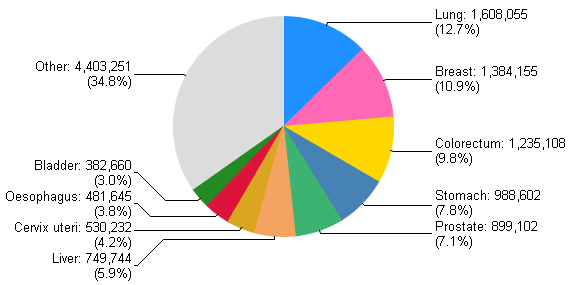
\includegraphics[width=.4\textwidth]{./images/statistics/repartitionCancerIncidence.png}}%
      \hfill%
      \subfigure[][\tiny \# of cancer deaths]{%
        \label{fig:stat1b}%
        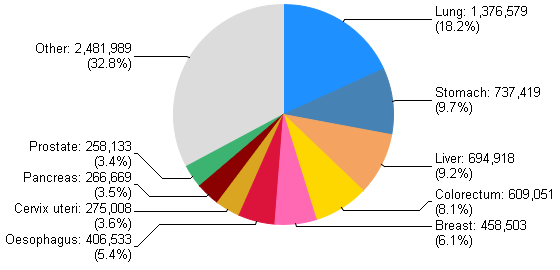
\includegraphics[width=.4\textwidth]{./images/statistics/repartitionCancerDeaths.png}}%
      \hspace*{\fill}%
      \label{fig:stat1}%
      % \caption{Statistics regarding cancer in 2008~\footnotemark}
    \end{figure}
  \end{block}
  \begin{block}{\small Implications, image source\footnotemark}\scriptsize
    \begin{itemize}
    \item 2\textsuperscript{nd} most frequently diagnosed men cancer
    \item Accounting for $7.1\%$ of overall cancers diagnosed
    \item Accounting for $3.4\%$ of overall cancers death
    \end{itemize}
  \end{block}
  \footcitetext{Ferlay2010}
\end{frame}

\subsection{The prostate organ}

\begin{frame}
  \frametitle{Introduction}
  \framesubtitle{The prostate organ}
  \begin{block}{\small Anatomy}
    \begin{figure}%
      \centering
      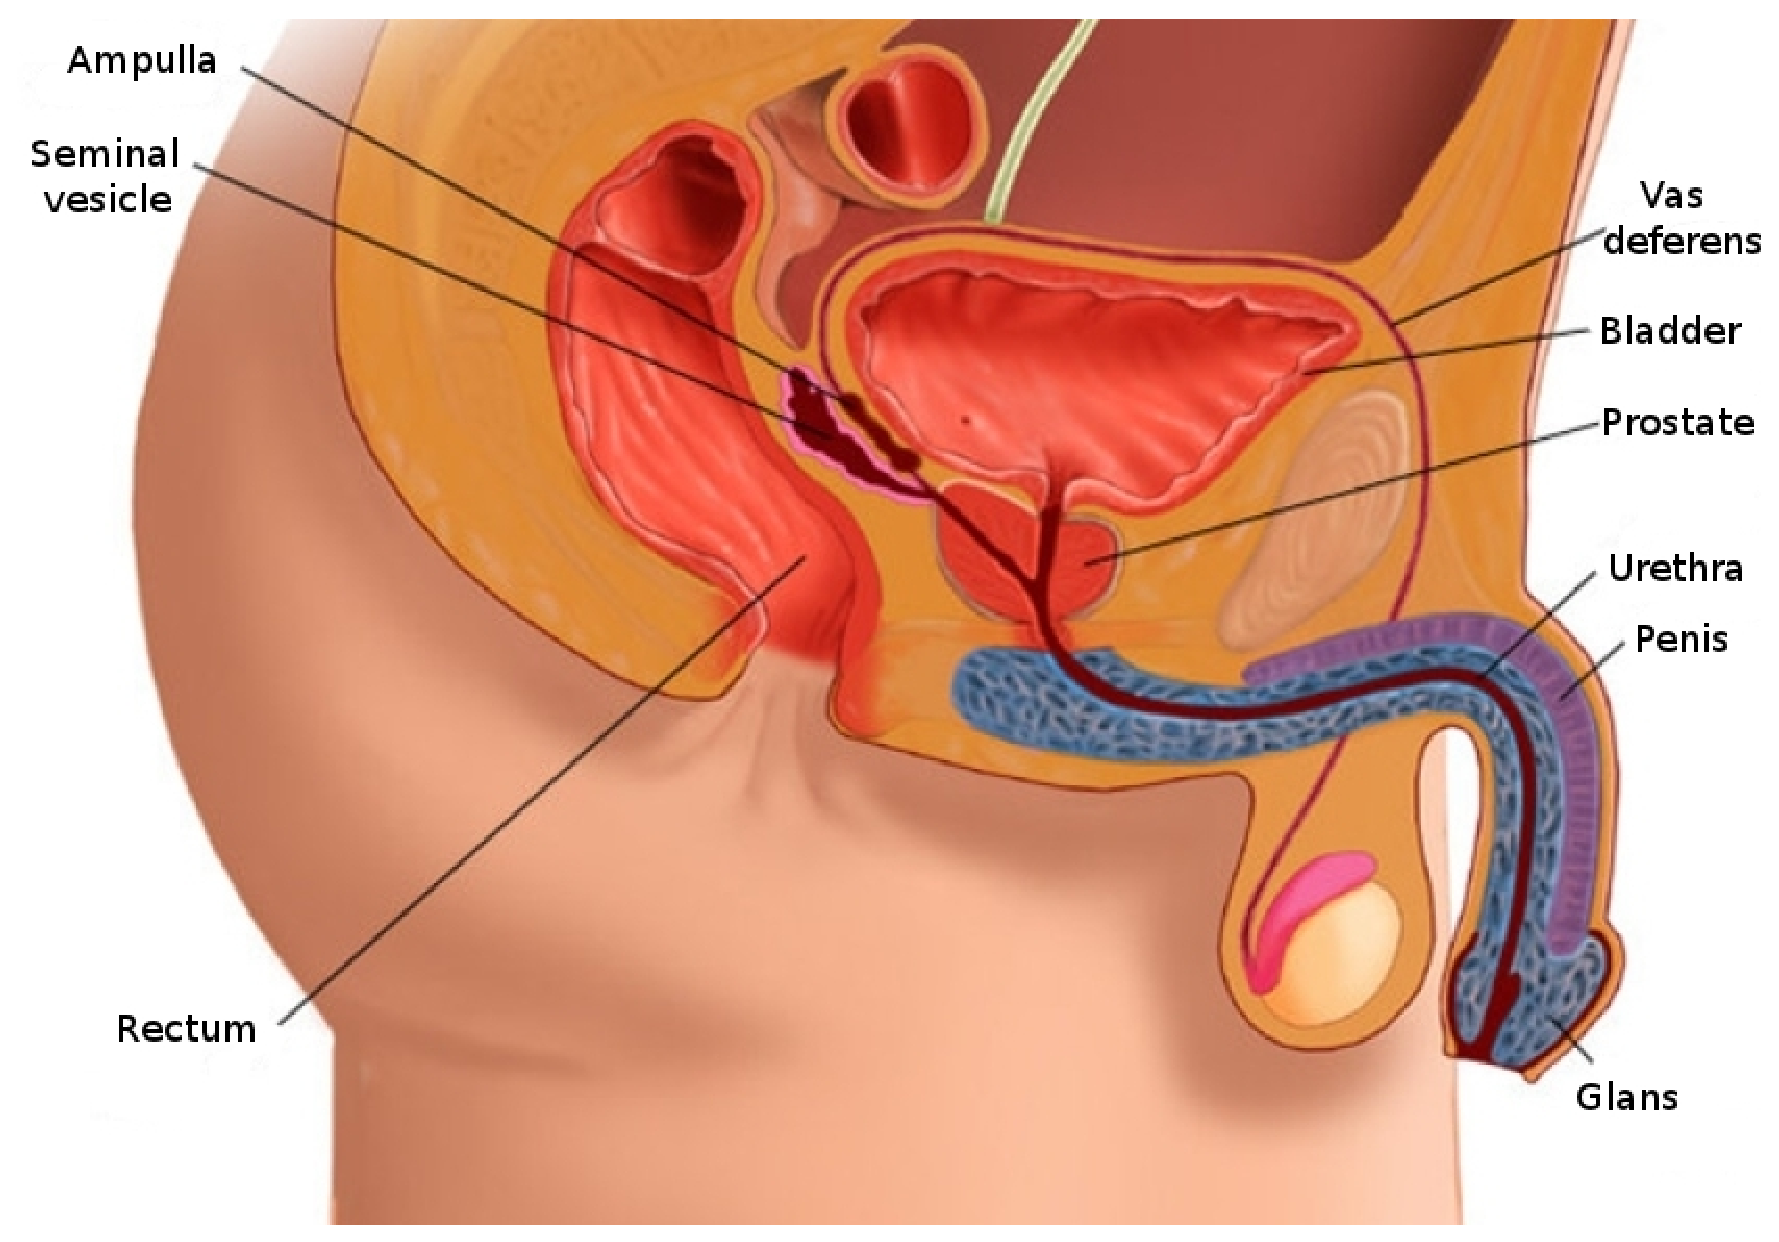
\includegraphics[height=.3\textheight]{./images/anatomy/prostate2D.eps}
      \caption{\tiny Localization of the prostate organ, image source\footnotemark}
    \end{figure}
  \end{block}
  \begin{block}{\small Characteristics}\scriptsize
    \begin{itemize}
    \item Height: \SI{3}{\cm}
    \item Depth: \SI{2.5}{\cm}
    \item Weight: \SIrange{7}{16}{\g}
    \end{itemize}
  \end{block}
  \footcitetext{Geckomedia2011}
\end{frame}

\begin{frame}
  \frametitle{Introduction}
  \framesubtitle{The prostate organ}
  \begin{block}{\small Anatomy}
    \begin{figure}%
      \centering
      \hspace*{\fill}%
      \subfigure[][\tiny Transverse plane]{%
        \label{fig:stat1a}%
        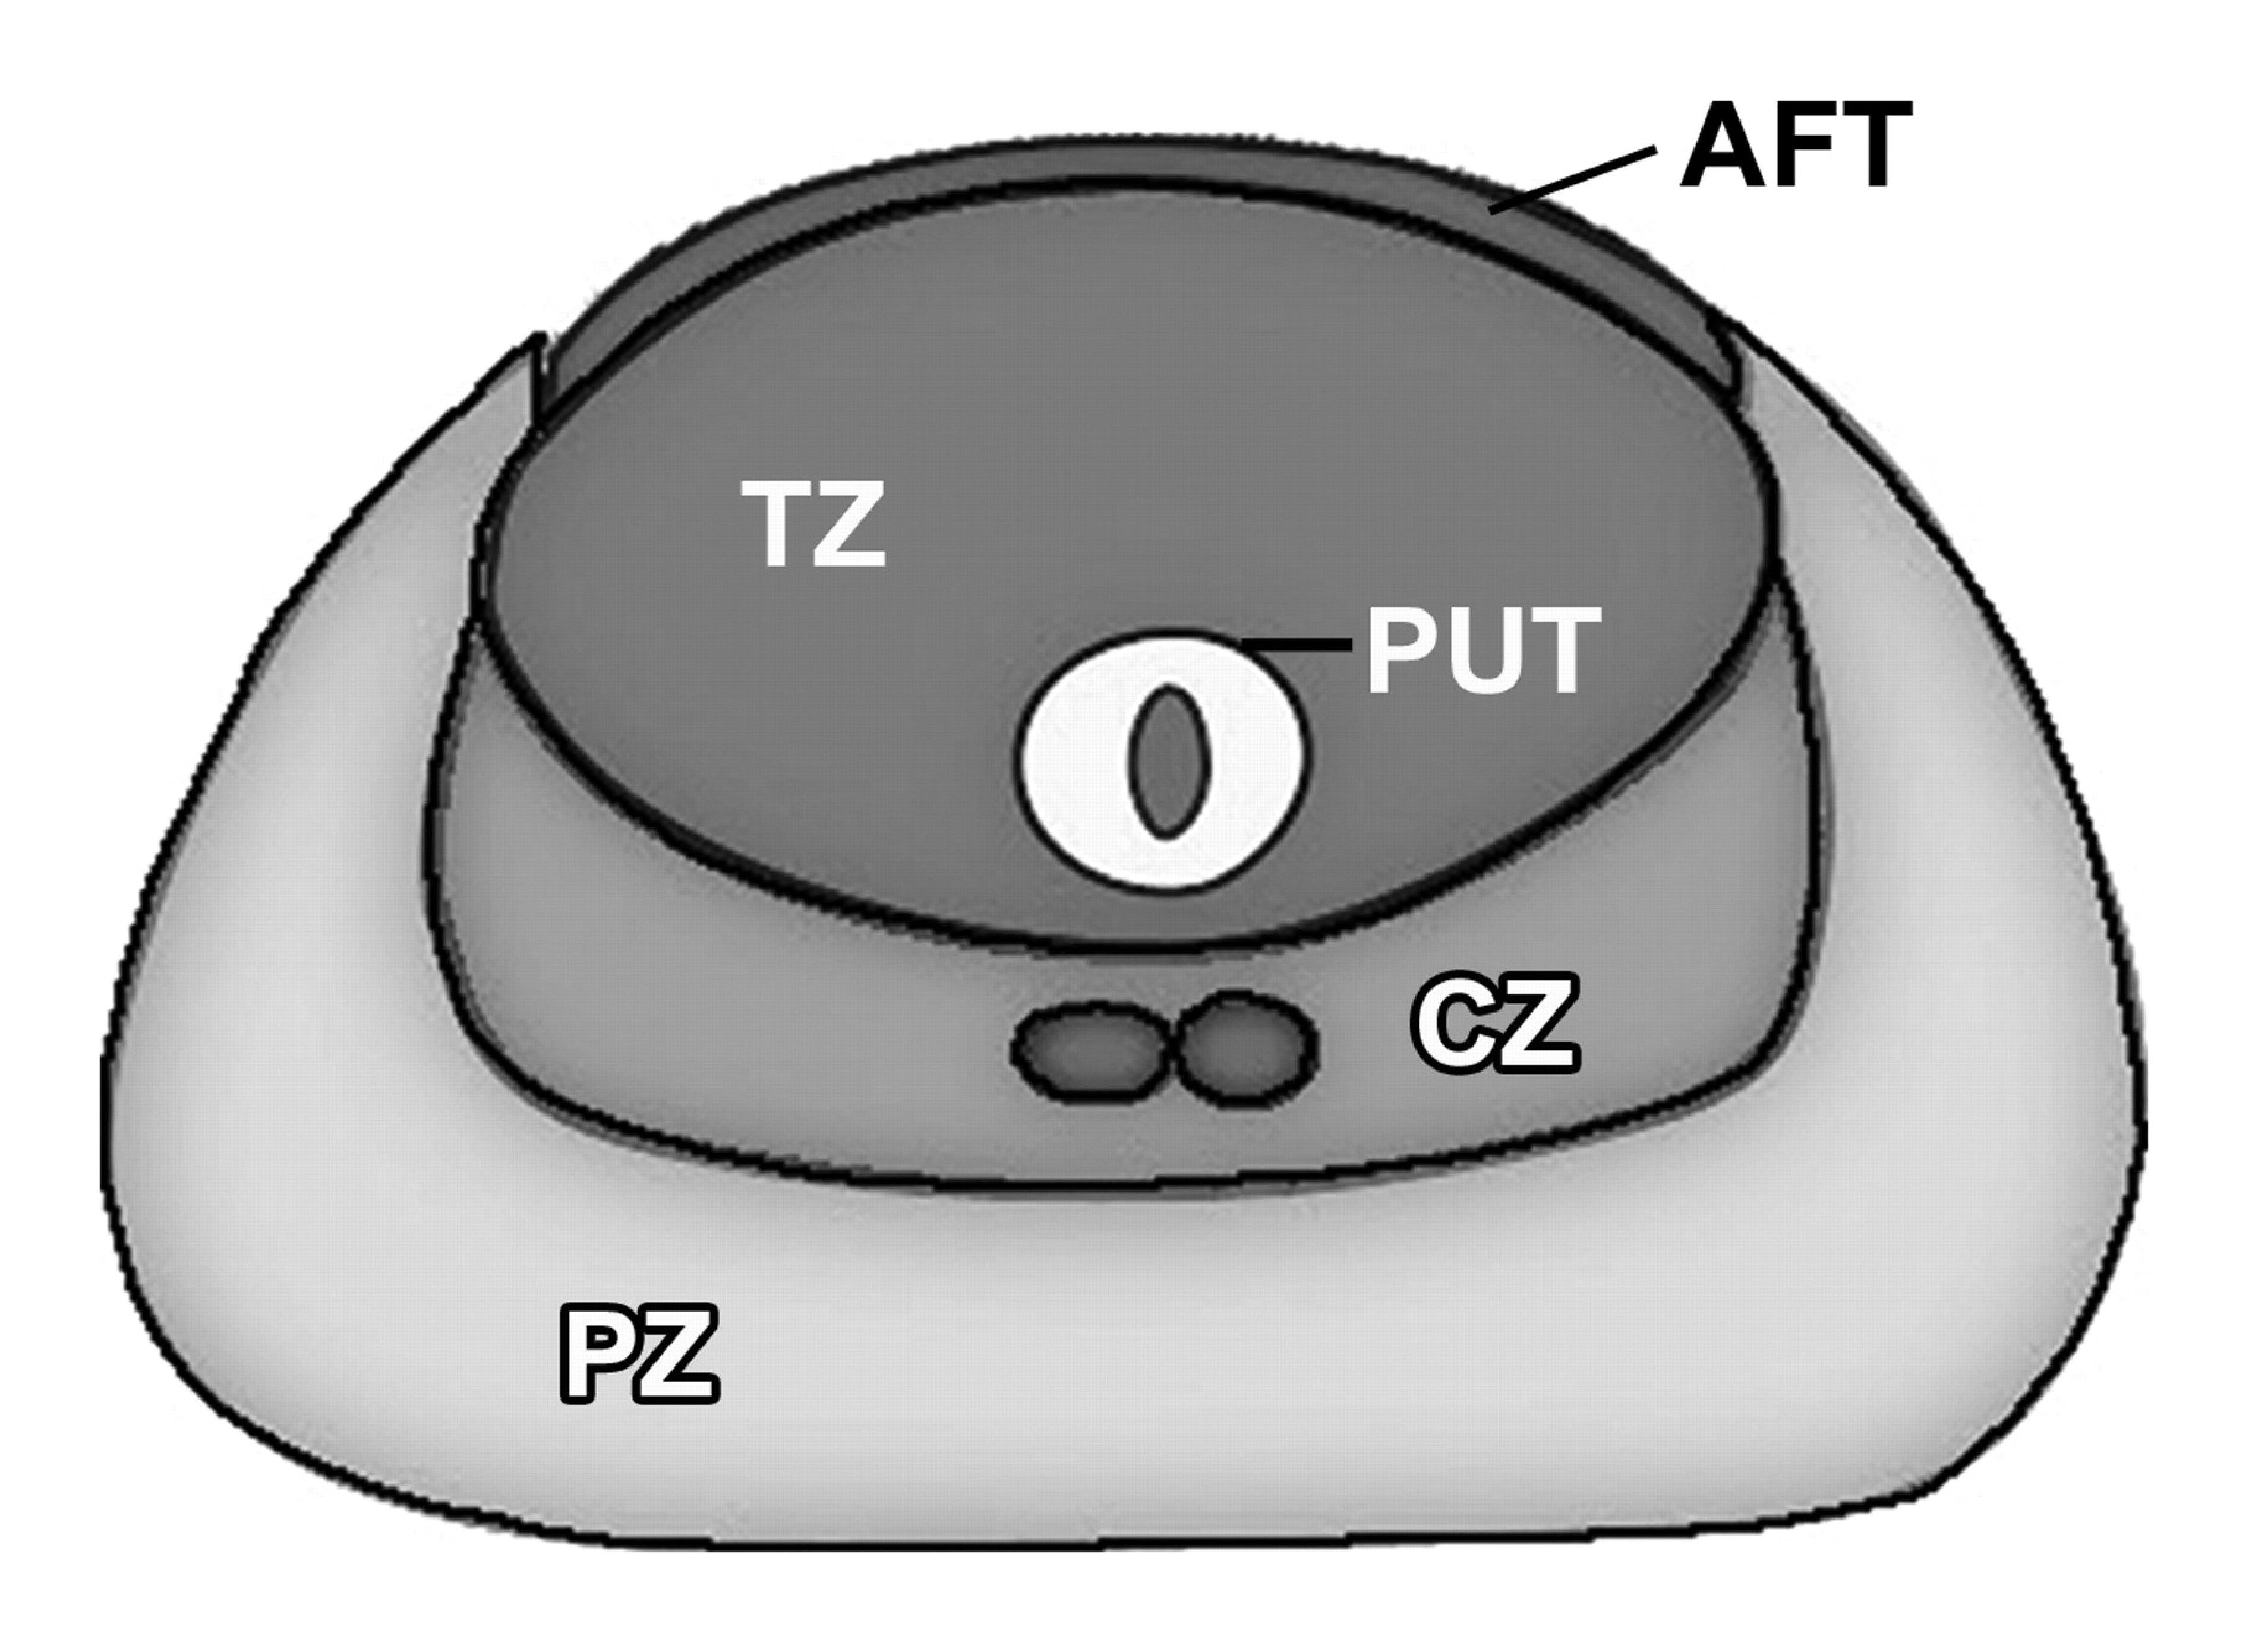
\includegraphics[height=.28\textheight]{./images/anatomy/prostateTransverse.eps}}%
      \hfill%
      \subfigure[][\tiny Sagittal plane]{%
        \label{fig:stat1b}%
        \includegraphics[height=.35\textheight]{./images/anatomy/prostateSagital.eps}}%
      \hspace*{\fill}%
      \caption{\tiny Prostate zones - AFT: anterior fibromuscular tissue, CZ: central zone, ED: ejaculatory duct, NVB: neurovascular bundle, PUT: periurethral tissue, PZ: peripheral zone, U: urethra, TZ: transitional zone, B: base, M: median, A: apex; image source\footnotemark}
      \label{fig:stat1}%
    \end{figure}
  \end{block}
  \footcitetext{Choi2007}
\end{frame}

\subsection{Prostate carcinoma}

\begin{frame}
  \frametitle{Introduction}
  \framesubtitle{Prostate carcinoma (CaP)}
  \begin{center}
    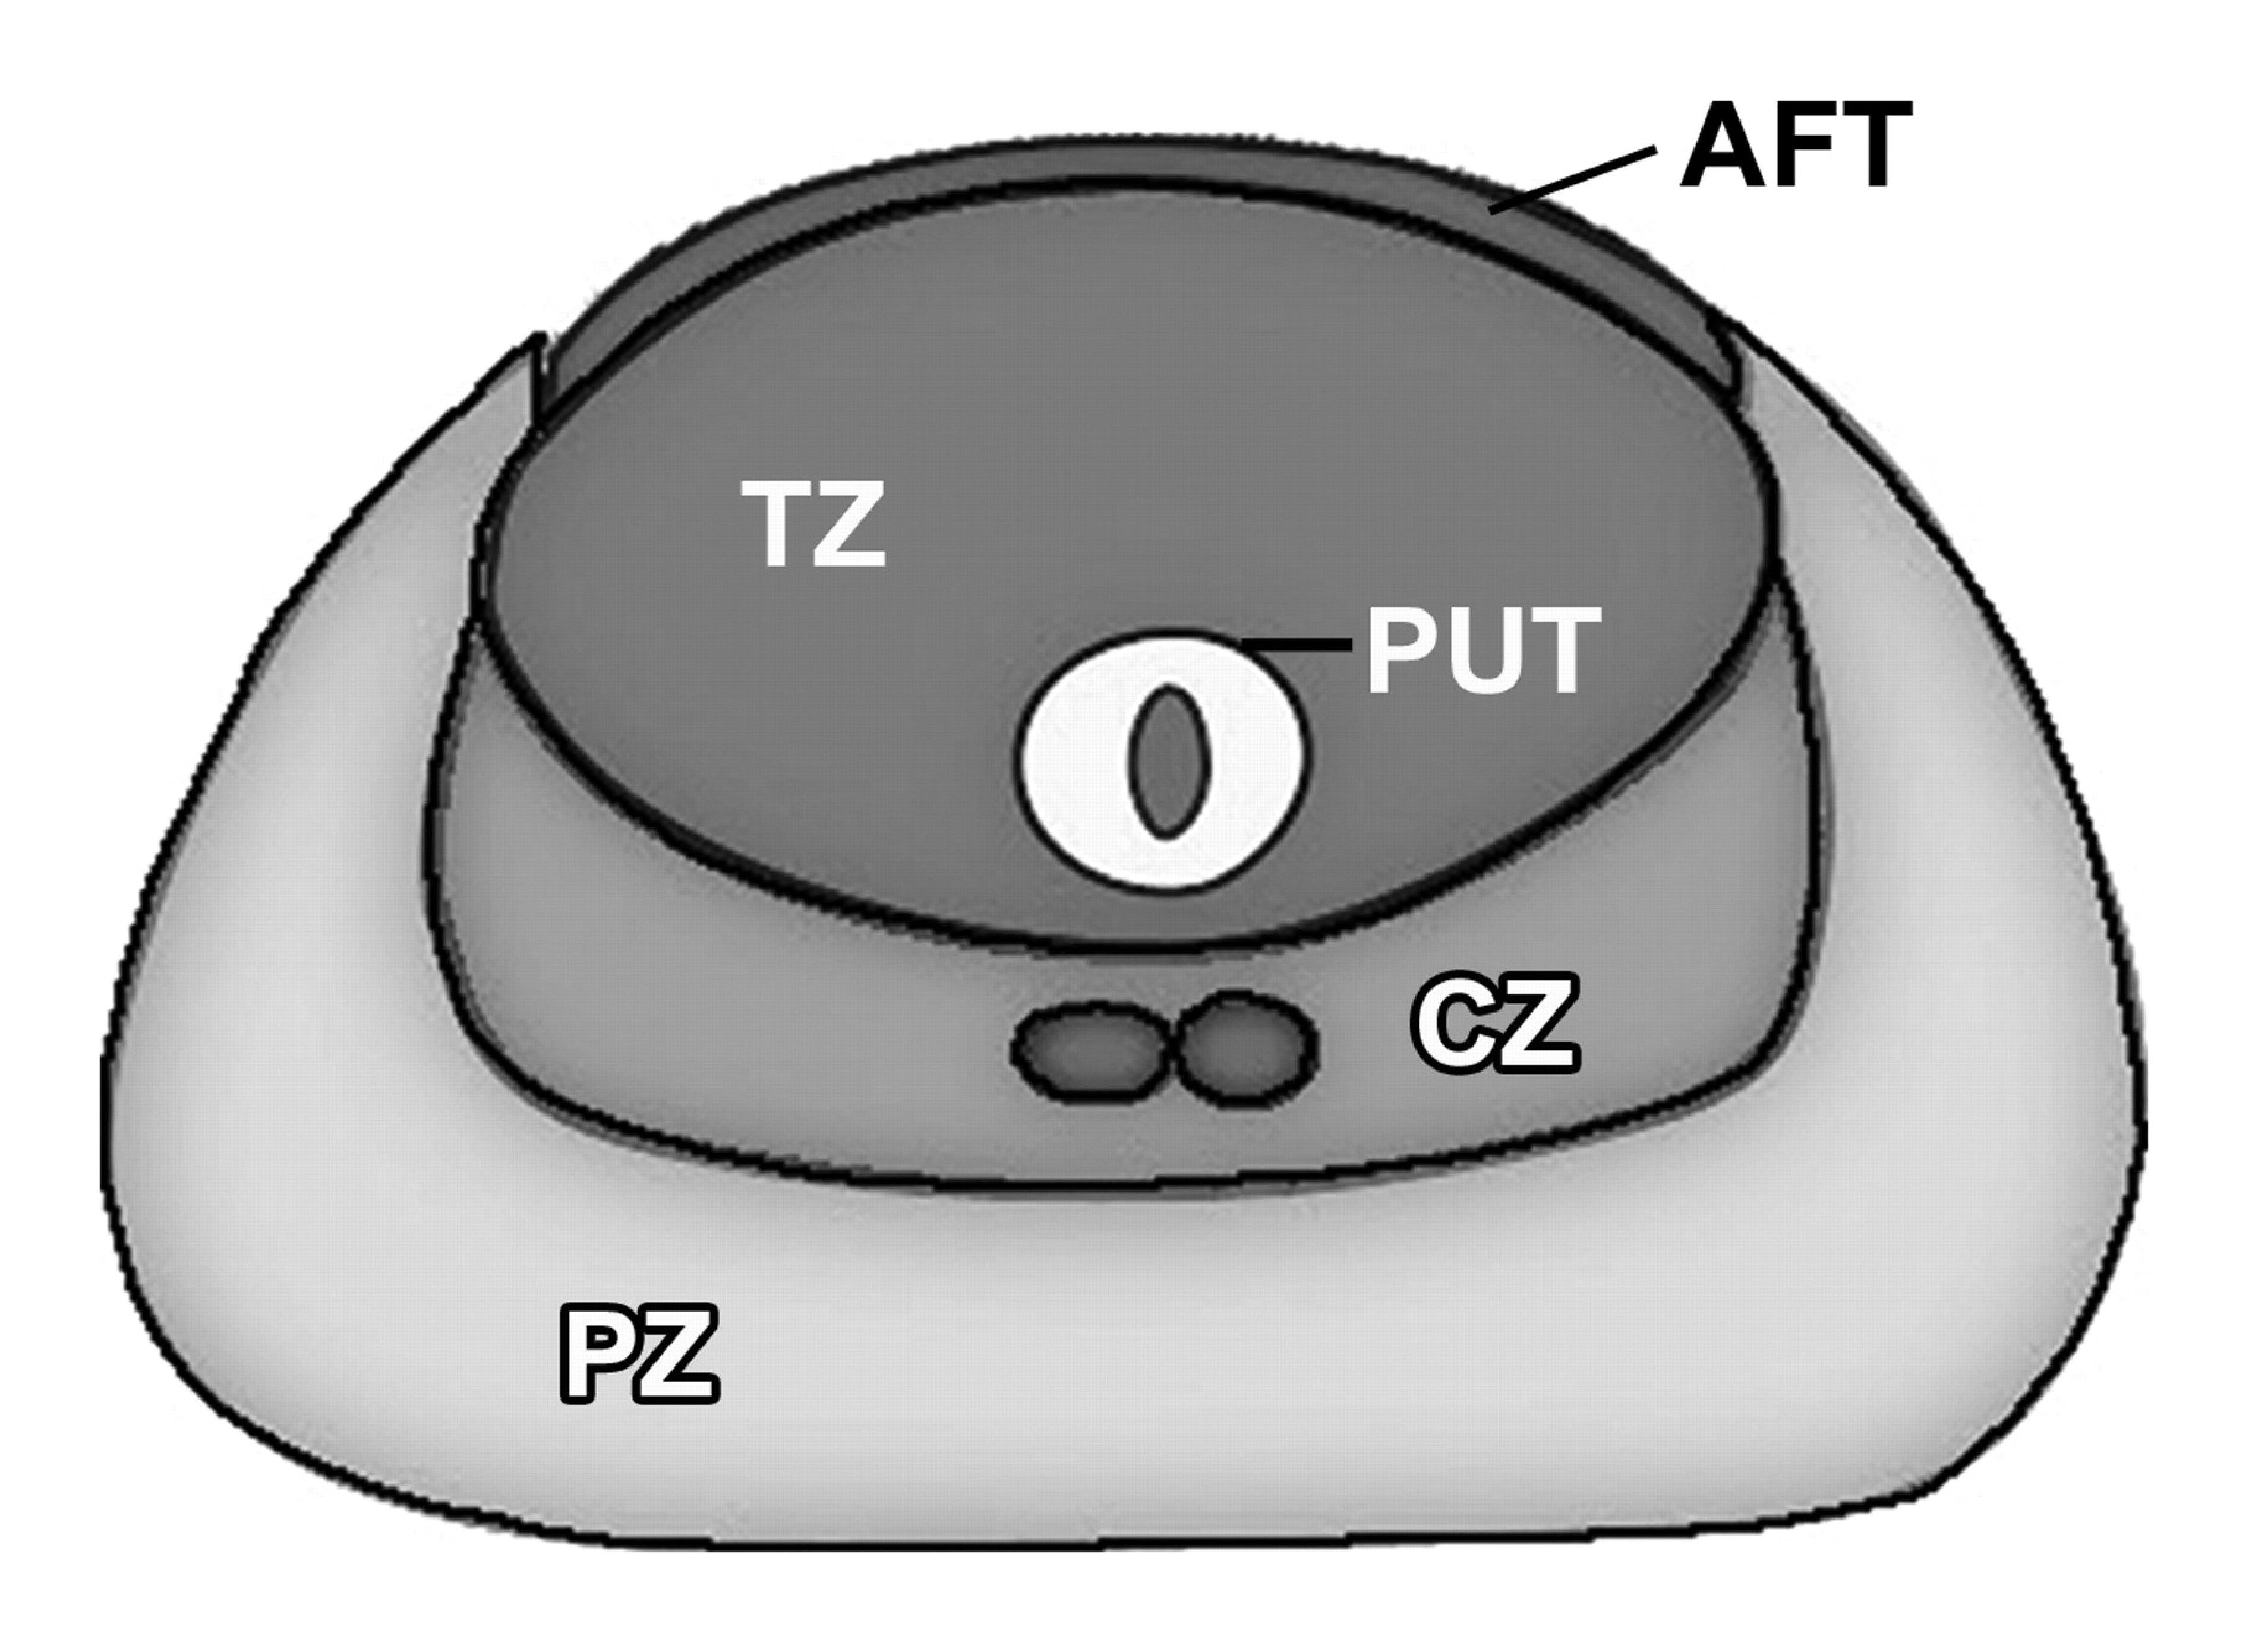
\includegraphics[height=.25\textheight]{./images/anatomy/prostateTransverse.eps}
  \end{center}
  \begin{columns}
    \begin{column}{0.45\textwidth}
      \begin{block}{\small CaP development}
        \begin{itemize}\scriptsize
        \item Slow-growing $\rightarrow$ \SI{85}{\percent}
        \item Fast-growing $\rightarrow$ \SI{15}{\percent}
        \item CaPs in CG are more aggressive
        \end{itemize}
      \end{block}
    \end{column}
    \begin{column}{0.45\textwidth}
      \begin{block}{\small Zonal predisposition}
        \begin{itemize}\scriptsize
        \item PZ $\rightarrow$ \SIrange{70}{80}{\percent}
        \item TZ $\rightarrow$ \SIrange{10}{20}{\percent}
        \item CG $\rightarrow$ \SI{5}{\percent}
        \end{itemize}
      \end{block}
    \end{column}
  \end{columns}
  \begin{greenblock}{\small Goals}
    \begin{itemize}\scriptsize
    \item Detect CaP
    \item Distinguish slow- from fast-growing CaP
    \item Active surveillance \emph{vs.} prostatectomy/other treatments
    \end{itemize}
  \end{greenblock}
\end{frame}

\subsection{Screening}

\begin{frame}
  \frametitle{Introduction}
  \framesubtitle{Screening}
  \begin{columns}
    \begin{column}{0.5\textwidth}
      \begin{block}<1->{\small Prostate-specific antigen}
        \begin{itemize}\scriptsize
        \item<1-> $>$ \SI{10}{\nano\gram\per\milli\liter} $\rightarrow$ biopsy
        \item<2-> From \SIrange{4}{10}{\nano\gram\per\milli\liter}
          \begin{itemize}\scriptsize
          \item[$\rightarrow$] $\frac{\text{\tikzbullet{gray}{orangeubfc}}}{\text{\tikzbullet{gray}{orangeubfc}}\  +\  \text{\tikzbullet{gray}{blueubfc}}} > 15 \% \rightarrow$ biopsy
          \end{itemize}
        \item[\cross]<3-> Not reliable
        \end{itemize}
      \end{block}
      \begin{block}<1->{\small ``Blind'' transrectal ultrasound biopsy}
        \begin{itemize}\scriptsize
          \item<4-> Take samples from different locations
          \item<4-> Grade using Gleason score
          \item[\cross]<5-> Invasive procedure
          \item[\cross]<5-> Lead to false positives \& negatives
        \end{itemize}
      \end{block}
    \end{column}
    \begin{column}{0.5\textwidth}
      \begin{center}
        \only<1>{
          \begin{figure}
          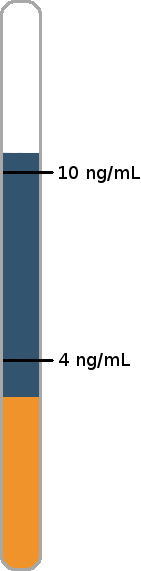
\includegraphics[height=.6\textheight]{./images/screening/high_psa.png}
          \caption{\tiny \tikzbullet{gray}{orangeubfc} free PSA \\ \tikzbullet{gray}{blueubfc} protein-linked PSA}
          \end{figure}
        }
        \only<2>{
          \begin{figure}
          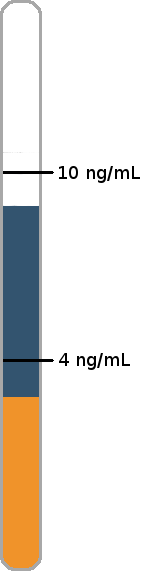
\includegraphics[height=.6\textheight]{./images/screening/risk_psa.png}
          \caption{\tiny \tikzbullet{gray}{orangeubfc} free PSA \\ \tikzbullet{gray}{blueubfc} protein-linked PSA}
          \end{figure}
        }
        \only<3>{
          \begin{figure}
          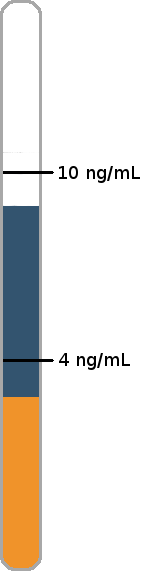
\includegraphics[height=.6\textheight]{./images/screening/risk_psa.png}
          \caption{\tiny \tikzbullet{gray}{orangeubfc} free PSA \\ \tikzbullet{gray}{blueubfc} protein-linked PSA}
          \end{figure}
        }
        \only<4>{
          \begin{figure}
          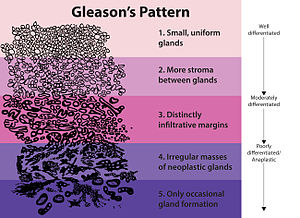
\includegraphics[height=.3\textheight]{./images/screening/gleason.jpg}
          \caption{\tiny Image source: \texttt{https://goo.gl/fEVQXQ}}
          \end{figure}
        }
        \only<5>{
          \begin{figure}
          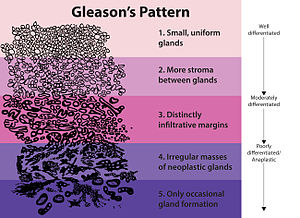
\includegraphics[height=.3\textheight]{./images/screening/gleason.jpg}
          \caption{\tiny Image source: \texttt{https://goo.gl/fEVQXQ}}
          \end{figure}
        }
        \only<6>{
          \begin{greenblock}{\small Pros}
            \begin{itemize}\scriptsize
            \item[\tick]<6-> Reduce CaP-related mortality from \SIrange{21}{44}{\percent}\footnotemark
            \end{itemize}
          \end{greenblock}
          \begin{redblock}{\small Cons}
            \begin{itemize}\scriptsize
            \item[\cross] Up to \SI{30}{\percent} of over-diagnosis\footnotemark
            \item[\cross] Up to \SI{35}{\percent} of undiagnosed CaP\footnotemark
            \item[\cross] Biopsies are invasive
            \end{itemize}
          \end{redblock}}
      \end{center}
    \end{column}
    \only<6>{\addtocounter{footnote}{-3} \stepcounter{footnote} \footcitetext{Schroeder2012} \stepcounter{footnote} \footcitetext{Haas2007} \stepcounter{footnote} \footcitetext{Taira2010}}
  \end{columns}
\end{frame}

\subsection{CAD and mp-MRI}

\begin{frame}
  \frametitle{Introduction}
  \framesubtitle{CAD and mp-MRI}
  \begin{greenblock}{\small Current trendy techniques: mp-MRI}
    \begin{itemize}\scriptsize
    \item[\tick] Less invasive technique
    \end{itemize}
  \end{greenblock}
  \begin{redblock}{\small Human diagnosis using mp-MRI}
    \begin{itemize}\scriptsize
    \item[\cross] Need further investigation of the mp-MRI modalities
    \item[\cross] Low repeatability
      \begin{itemize} \scriptsize
        \item Observer limitations
        \item Complexity of clinical cases
      \end{itemize}
    \end{itemize}
  \end{redblock}
  \begin{block}{\small Emergence of CAD}
    \begin{itemize}\scriptsize
      \item CADe $\rightarrow$ detection of potential lesions
      \item CADx $\rightarrow$ diagnosis regarding those lesions
    \end{itemize}
  \end{block}
\end{frame}

\subsection{Research objectives}

\begin{frame}
  \frametitle{Introduction}
  \framesubtitle{Research objectives}
  \begin{block}{\small Propose a mp-MRI CAD for CaP}
    \begin{itemize}\scriptsize
      \item Study and investigate the state-of-the-art on MRI CAD for CaP
      \item Identify the scientific barriers
      \item Design a mp-MRI CAD addressing these issues
      \item Investigate and analyze the proposed CAD
    \end{itemize}
  \end{block}
\end{frame}

\section{CAD and mp-MRI}

\begin{frame}
    \tableofcontents[currentsection,currentsubsection,subsectionstyle=show/show/hide]
\end{frame}

\subsection{MRI modalities}

\setcounter{subfigure}{0}% Reset subfigure counter

\begin{frame}
  \frametitle{Introduction}
  \framesubtitle{MRI modalities}
  \begin{block}{\small T$_2$W-MRI}
    \begin{figure}%
      \centering
      \hspace*{\fill}%
      \subfigure[][\tiny Healthy]{%
        \label{fig:t2wh}%
        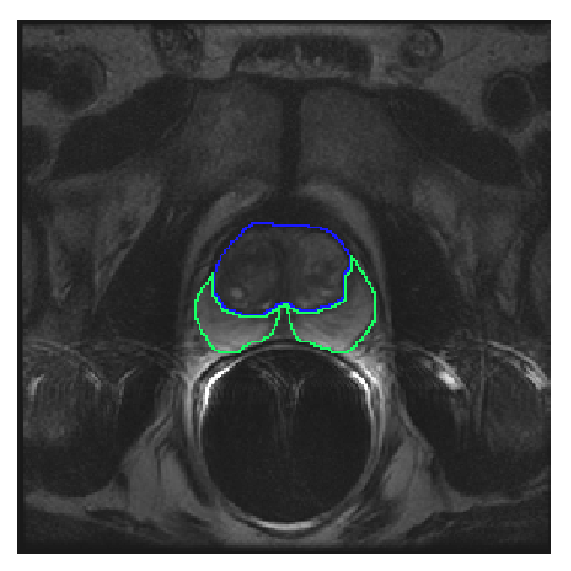
\includegraphics[width=.2\textwidth]{./images/mri/t2w/t2w_healthy.eps}}%
      \hfill%
      \subfigure[][\tiny CaP PZ]{%
        \label{fig:t2wcpz}%
        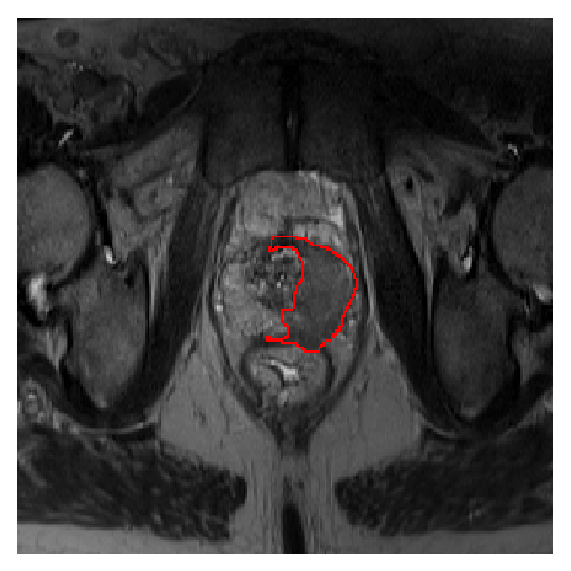
\includegraphics[width=.2\textwidth]{./images/mri/t2w/t2w_cancer_pz.eps}}%
      \hfill%
      \subfigure[][\tiny CaP CG]{%
        \label{fig:t2wccg}%
        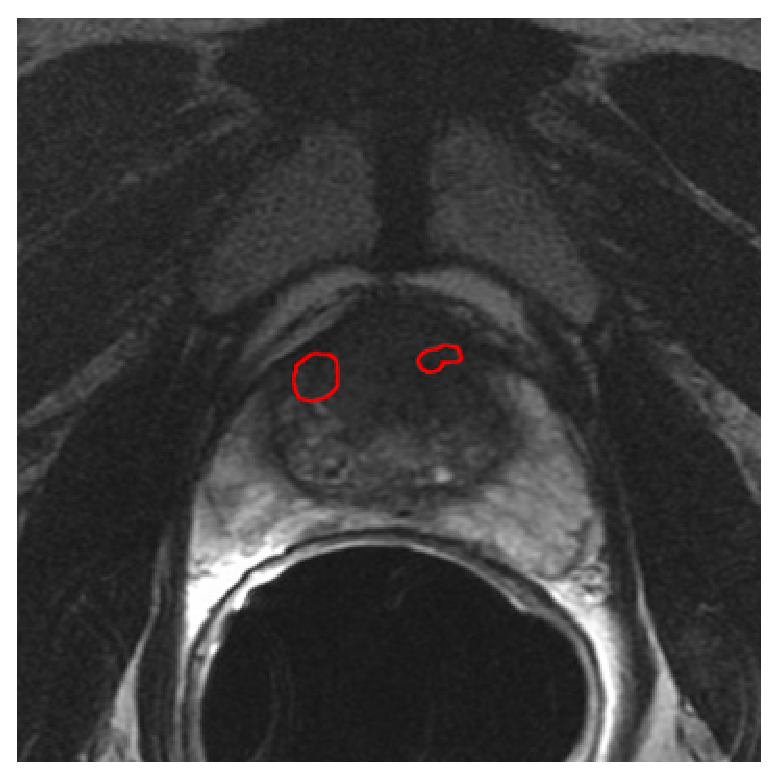
\includegraphics[width=.2\textwidth]{./images/mri/t2w/t2w_cancer_cg.eps}}%
      \hspace*{\fill}%
      \label{fig:t2w}%
    \end{figure}
  \end{block}
  \only<1>{
  \begin{columns}
    \begin{column}{0.5\textwidth}
      \begin{greenblock}{\small Healthy}\footnotesize
        \begin{itemize}\scriptsize
        \item Intermediate to high-signal intensity (SI) in PZ
        \item Low-SI in CG
        \end{itemize}
      \end{greenblock}
    \end{column}
    \begin{column}{0.5\textwidth}
      \begin{redblock}{\small CaP}\footnotesize
        \begin{itemize}\scriptsize
        \item Low-SI
        \item Round and ill-defined mass in PZ
        \item Homogeneous with ill-defined edges in CG
        \end{itemize}
      \end{redblock}
    \end{column}
  \end{columns}}
\only<2>{
  \begin{columns}
    \begin{column}{0.5\textwidth}
      \begin{greenblock}{\small Pros}\footnotesize
        \begin{itemize}\scriptsize
        \item Highest spatial resolution
        \item Anatomy nicely depicted
        \end{itemize}
      \end{greenblock}
    \end{column}
    \begin{column}{0.5\textwidth}
      \begin{redblock}{\small Cons}\footnotesize
        \begin{itemize}\scriptsize
        \item Low sensitivity in CG
        \item Lower specificity due to outliers
        \end{itemize}
      \end{redblock}
    \end{column}
  \end{columns}}
\end{frame}

\setcounter{subfigure}{0}% Reset subfigure counter

\begin{frame}
  \frametitle{Introduction}
  \framesubtitle{MRI modalities}
  \begin{block}{\small DCE-MRI}
    \begin{figure}%
      \centering
      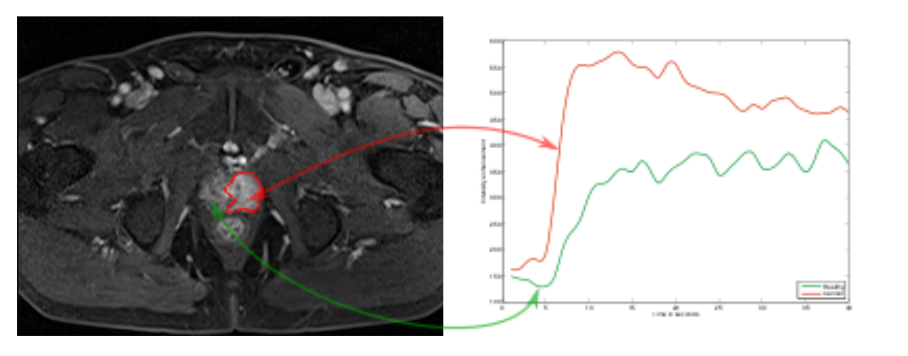
\includegraphics[width=.7\textwidth]{./images/mri/dce/dce_cancer_healthy_information.eps}
      \label{fig:dce}%
      \caption{{\color{green}Green}: healthy - {\color{red}Red}: CaP}
    \end{figure}
  \end{block}
  \only<1>{
  \begin{columns}
    \begin{column}{0.5\textwidth}
      \begin{greenblock}{\small Healthy}
        \begin{itemize}\scriptsize
        \item Slower wash-in, wash-out, time-to-peak enhancement
        \item Lower integral under the curve, max SI
        \end{itemize}
      \end{greenblock}
    \end{column}
    \begin{column}{0.5\textwidth}
      \begin{redblock}{\small CaP}
        \begin{itemize}\scriptsize
        \item Faster wash-in, wash-out, time-to-peak enhancement
        \item Higher integral under the curve, max SI
        \end{itemize}
      \end{redblock}
    \end{column}
  \end{columns}}
\only<2>{
  \begin{columns}
    \begin{column}{0.5\textwidth}
      \begin{greenblock}{\small Pros}\footnotesize
        \begin{itemize}\scriptsize
        \item Information about vascularity
        \end{itemize}
      \end{greenblock}
    \end{column}
    \begin{column}{0.5\textwidth}
      \begin{redblock}{\small Cons}\footnotesize
        \begin{itemize}\scriptsize
        \item Spatial mis-registration
        \item Lower spatial resolution than T$_2$W-MRI
        \item Difficult detection in CG
        \end{itemize}
      \end{redblock}
    \end{column}
  \end{columns}}
\end{frame}

\setcounter{subfigure}{0}% Reset subfigure counter

\begin{frame}
  \frametitle{Introduction}
  \framesubtitle{MRI modalities}
  \begin{block}{\small DW-MRI - ADC}
    \begin{figure}%
      \centering
      \hspace*{\fill}%
      \subfigure[][\tiny DW MRI]{%
        \label{fig:dw}%
        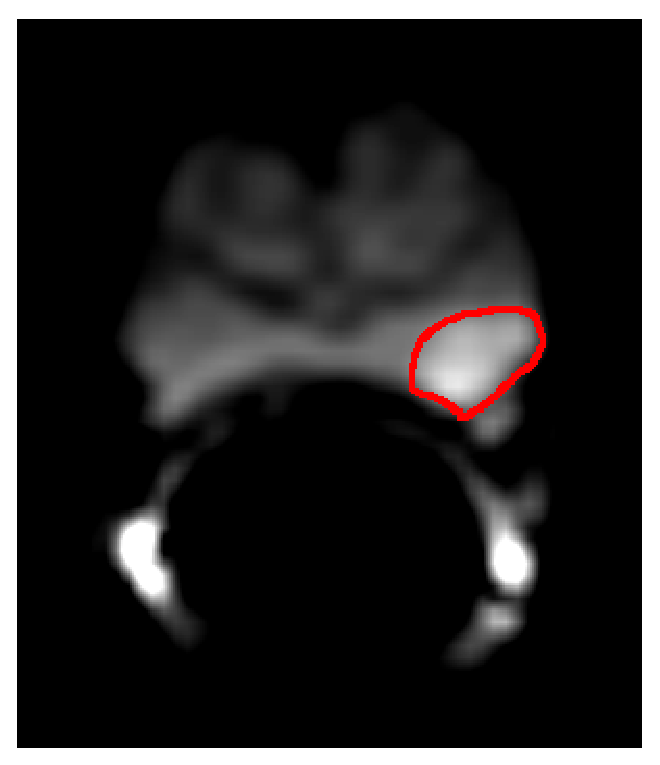
\includegraphics[width=.2\textwidth]{./images/mri/dwi/dwi_cancer.eps}}%
      \hfill%
      \subfigure[][\tiny ADC]{%
        \label{fig:adc}%
        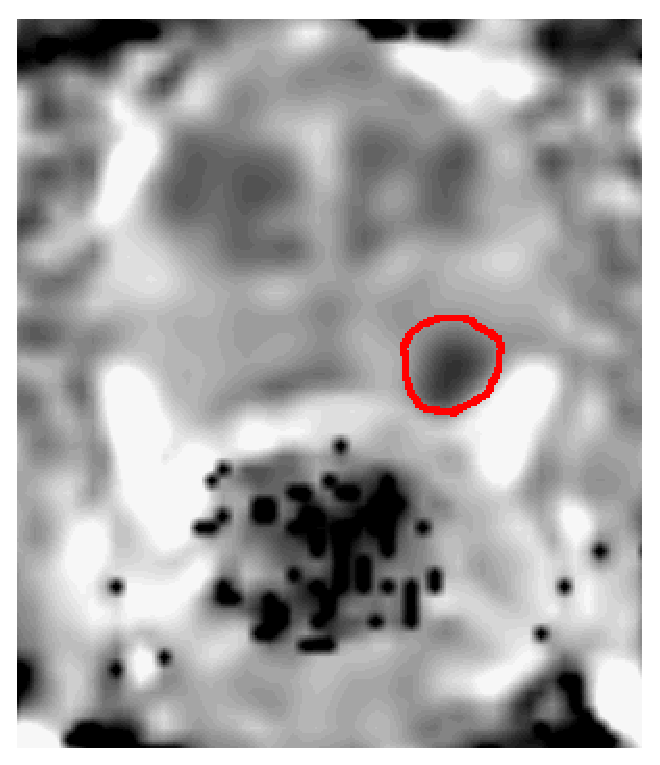
\includegraphics[width=.2\textwidth]{./images/mri/dwi/adc_cancer.eps}}%
      \hspace*{\fill}%
      \label{fig:dwadc}%
    \end{figure}
  \end{block}
  \only<1>{
  \begin{columns}
    \begin{column}{0.5\textwidth}
      \begin{greenblock}{\small Healthy}
        \begin{itemize}\scriptsize
        \item DW-MRI: lower SI
        \item ADC: higher-SI
        \end{itemize}
      \end{greenblock}
    \end{column}
    \begin{column}{0.5\textwidth}
      \begin{redblock}{\small CaP}\scriptsize
        \begin{itemize}
        \item DW-MRI: higher SI
        \item ADC: lower-SI
        \end{itemize}
      \end{redblock}
    \end{column}
  \end{columns}}
  \only<2>{
  \begin{columns}
    \begin{column}{0.5\textwidth}
      \begin{greenblock}{\small Pros}
        \begin{itemize}\scriptsize
        \item Information about tissue structure
        \item ADC correlated with Gleason score
        \end{itemize}
      \end{greenblock}
    \end{column}
    \begin{column}{0.5\textwidth}
      \begin{redblock}{\small Cons}\scriptsize
        \begin{itemize}
        \item Poor spatial resolution
        \item Variability of the ADC coefficient
        \end{itemize}
      \end{redblock}
    \end{column}
  \end{columns}}
\end{frame}

\setcounter{subfigure}{0}% Reset subfigure counter

\begin{frame}
  \frametitle{Introduction}
  \framesubtitle{MRI modalities}
  \begin{block}{\small MRSI}
    \begin{figure}%
      \centering
      \hspace*{\fill}%
      \subfigure[][\tiny Healthy]{%
        \label{fig:mrsih}%
        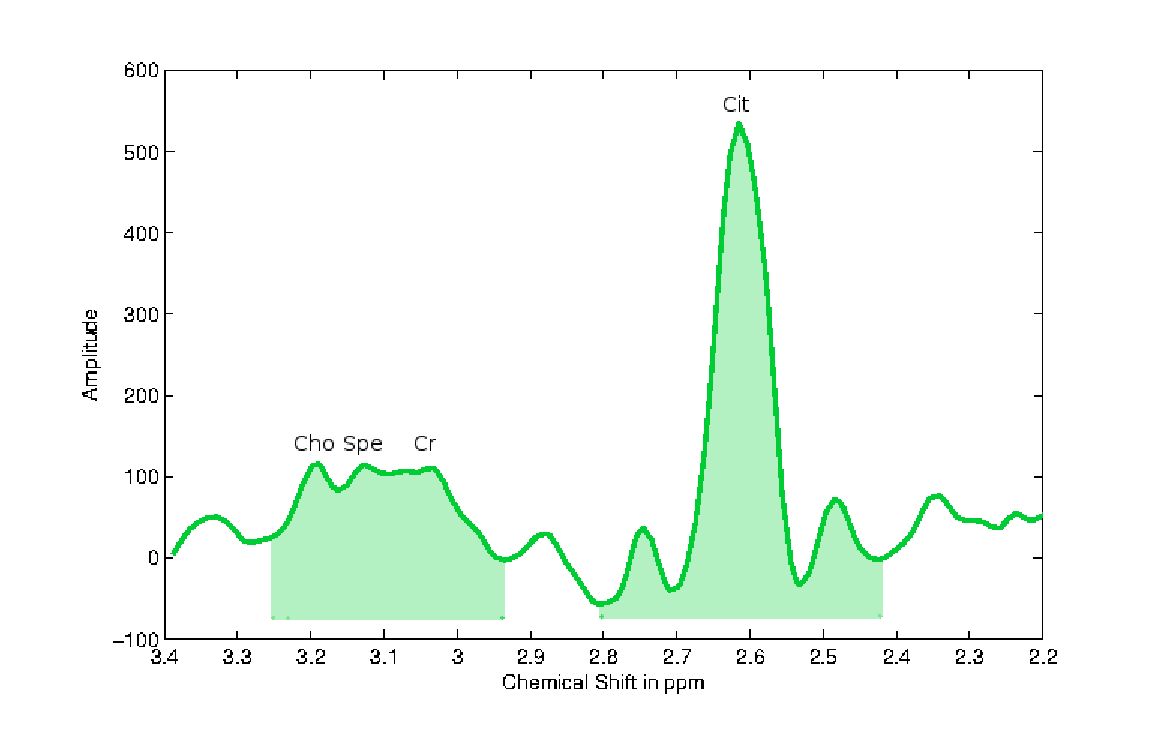
\includegraphics[width=.45\textwidth]{./images/mri/mrsi/mrsi_healthy.eps}}%
      \hfill%
      \subfigure[][\tiny CaP]{%
        \label{fig:mrsic}%
        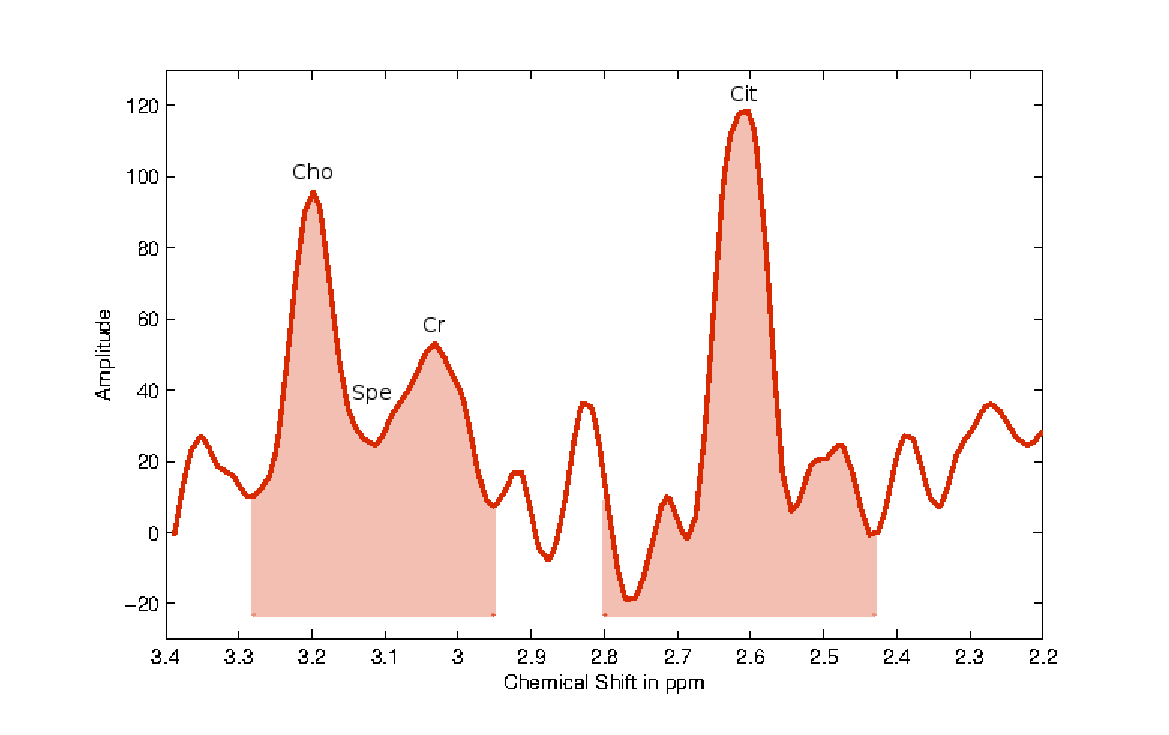
\includegraphics[width=.45\textwidth]{./images/mri/mrsi/mrsi_cancer.eps}}%
      \hspace*{\fill}%
      \label{fig:mrsi}%
    \end{figure}
  \end{block}
  \only<1>{
  \begin{columns}
    \begin{column}{0.5\textwidth}
      \begin{greenblock}{\small Healthy}
        \begin{itemize}\scriptsize
        \item High citrate
        \item Moderate choline and spermine
        \end{itemize}
      \end{greenblock}
    \end{column}
    \begin{column}{0.5\textwidth}
      \begin{redblock}{\small CaP}
        \begin{itemize}\scriptsize
        \item Decrease of citrate and spermine
        \item Increase of choline
        \end{itemize}
      \end{redblock}
    \end{column}
  \end{columns}}
\only<2>{
  \begin{columns}
    \begin{column}{0.5\textwidth}
      \begin{greenblock}{\small Pros}\footnotesize
        \begin{itemize}\scriptsize
        \item Citrate correlated with Gleason score
        \end{itemize}
      \end{greenblock}
    \end{column}
    \begin{column}{0.5\textwidth}
      \begin{redblock}{\small Cons}\footnotesize
        \begin{itemize}\scriptsize
        \item Low spatial resolution
        \item Variation inter-patients
        \end{itemize}
      \end{redblock}
    \end{column}
  \end{columns}}
\end{frame}

\subsection{The MedIA evil}

\begin{frame}
  \frametitle{The Medical Imaging evil}
  \begin{block}<1->{\small The reasons of a nightmare}\footnotesize
    \begin{itemize}
    \item[$\rightarrow$] Multidisciplinary competences: medical doctors vs. computer scientists
    \end{itemize}
  \end{block}
  \begin{redblock}<2->{\small Some examples}\footnotesize
    \begin{itemize}
    \item Delay in the data acquisition
    \item Interest differences between the different core competences
    \item[$\rightarrow$] Lack of interest
    \end{itemize}
  \end{redblock}
  \begin{greenblock}<3->{\small The keystones needed}\footnotesize
    \begin{itemize}
    \item Common datasets
    \item Algorithms comparisons
    \item Full benchmarking
    \end{itemize}
  \end{greenblock}
\end{frame}

\section{I2CVB}

\subsection{Overview}

\begin{frame}
  \frametitle{Overview}
  \begin{block}{
\includegraphics[height=.04\textheight]{./images/i2cvb/i2cvb.pdf}\ Platform}
    \begin{figure}
      \centering
      
\includegraphics[width=.8\linewidth]{./images/i2cvb/website.pdf}
    \end{figure}
    \begin{itemize}
    \item Development of a web platform
    \end{itemize}
  \end{block}
\end{frame}

\begin{frame}
  \frametitle{Manifesto}
  \begin{columns}
    \column{.5\textwidth}
    \begin{block}{
\includegraphics[height=.04\textheight]{./images/i2cvb/i2cvb.pdf}\ Vision}
      \begin{figure}
        \centering
        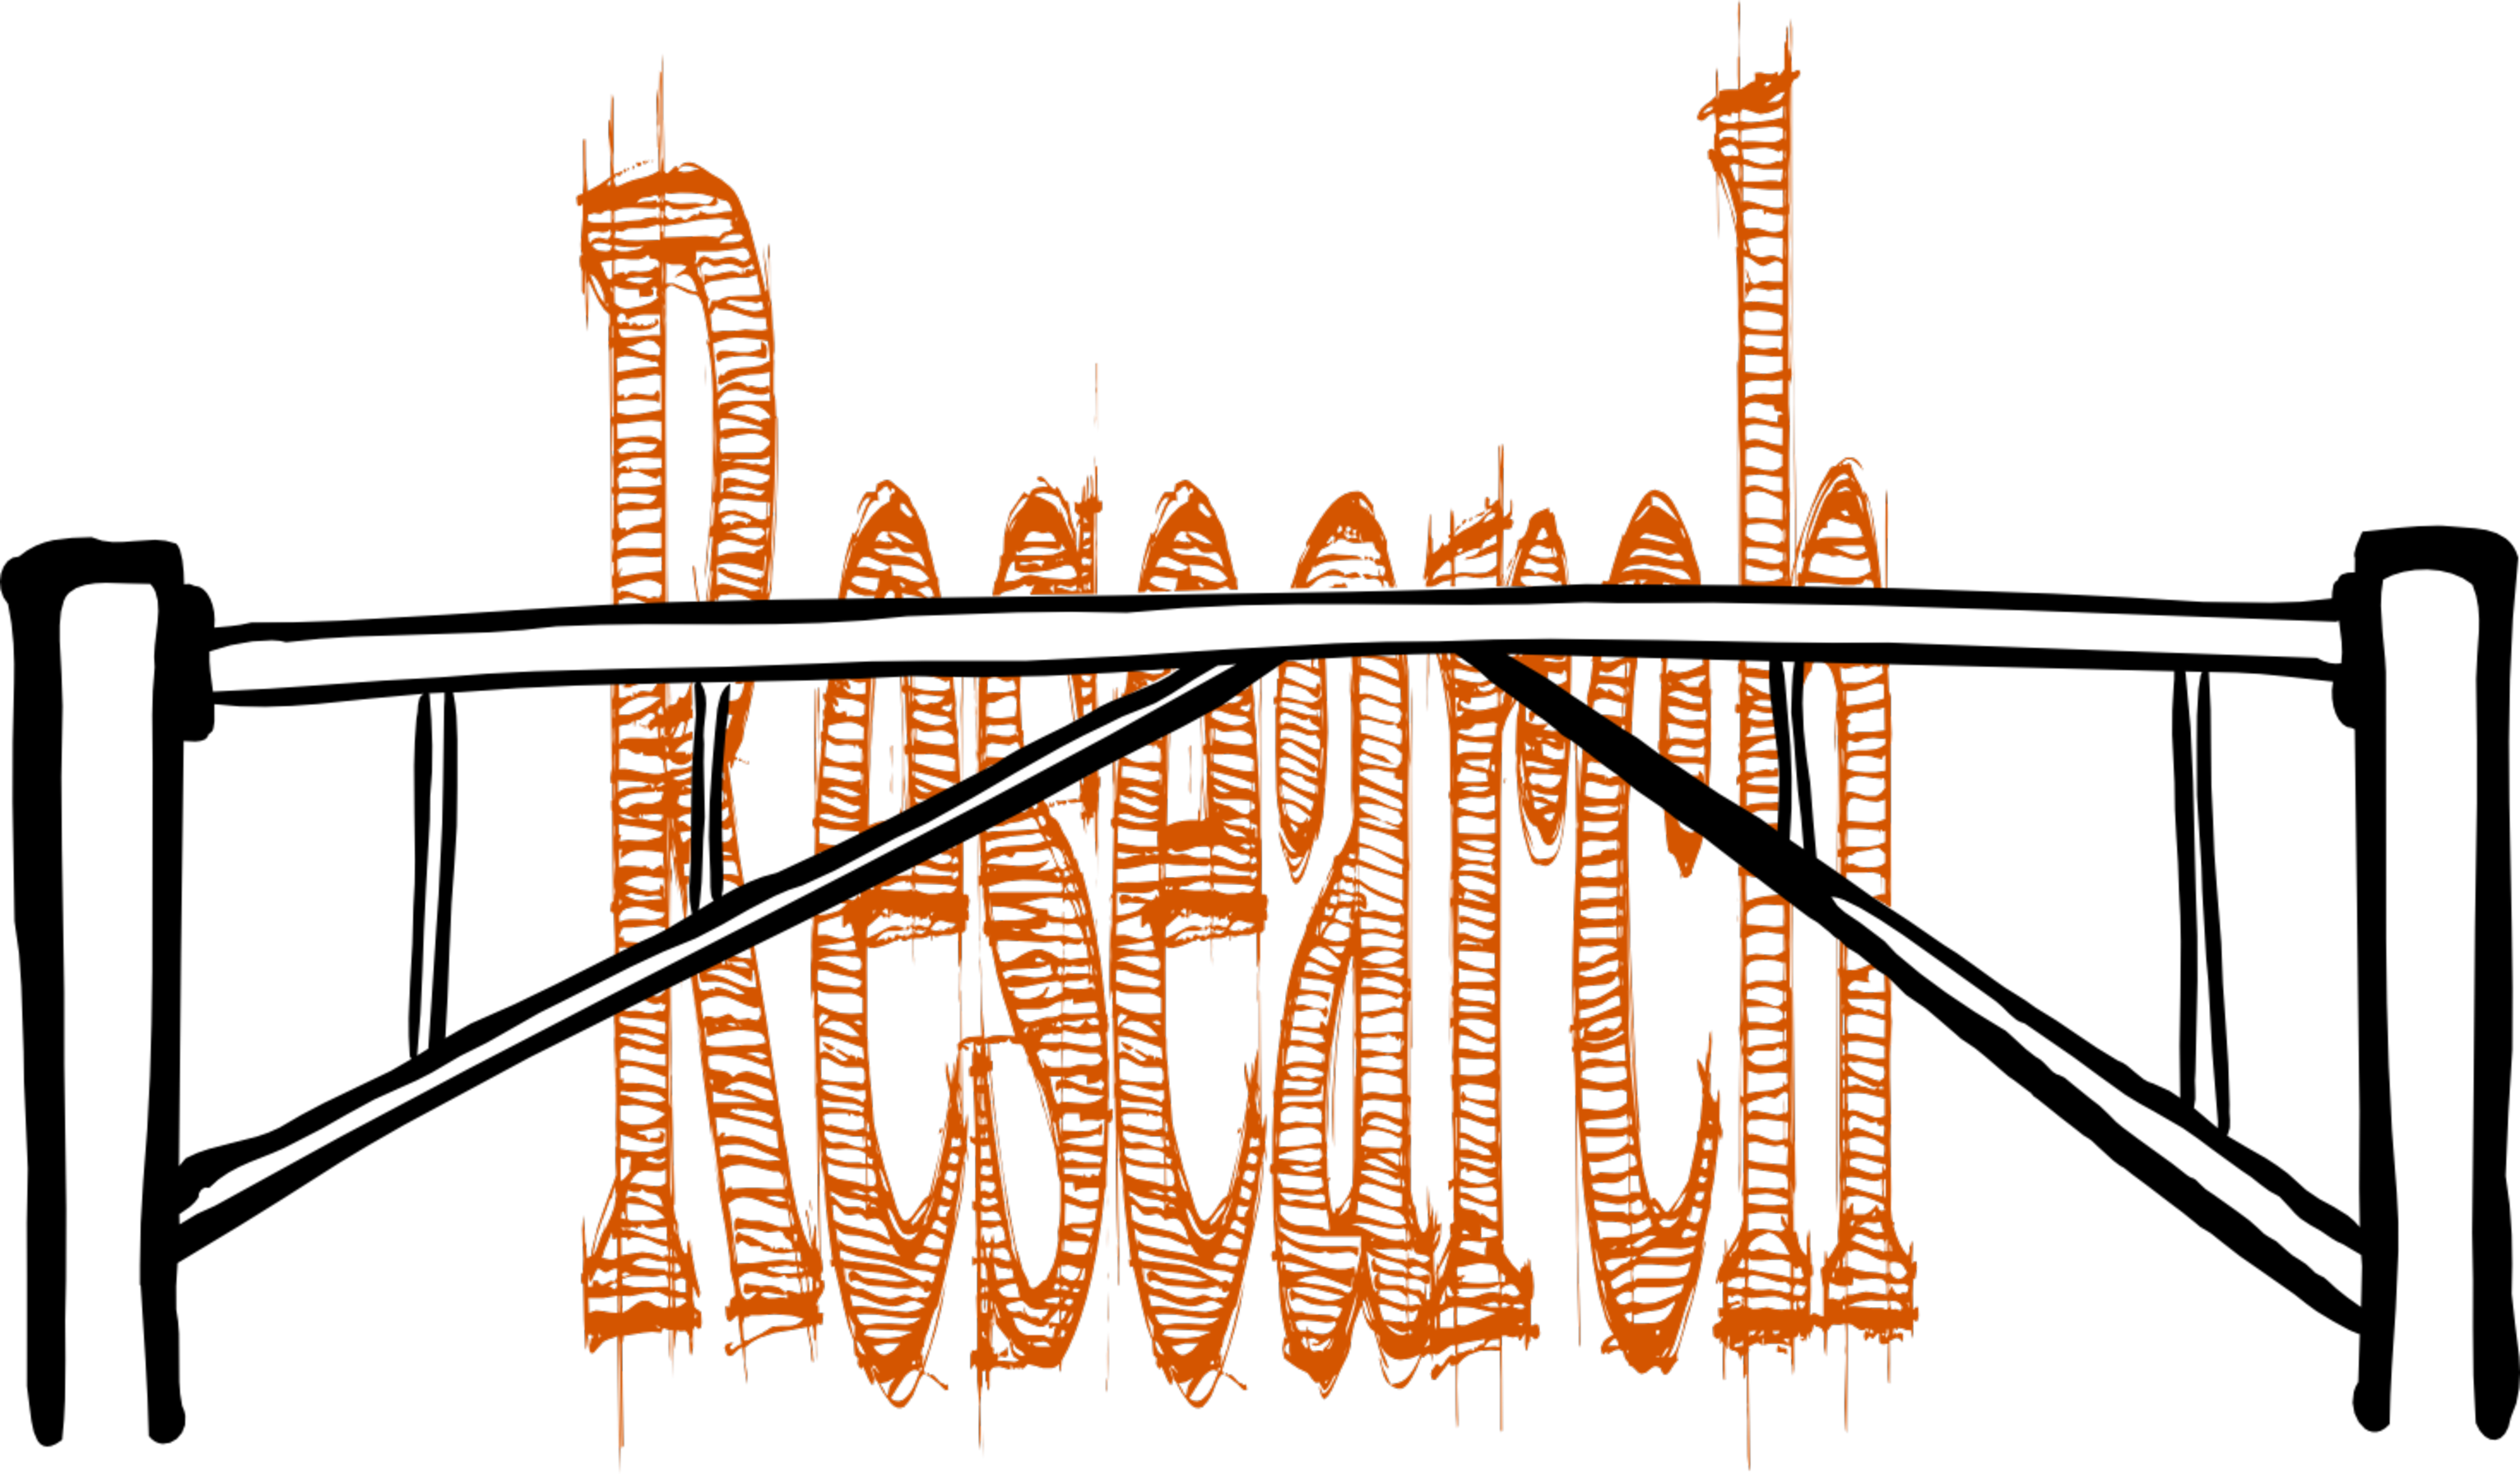
\includegraphics[height=.15\textheight]{./images/i2cvb/research.pdf}
      \end{figure}
      \vskip-4ex
      \begin{itemize}\tiny
      \item Democratization of the ability to research
      \end{itemize}
      \vskip1ex
    \end{block}
    \begin{block}{
\includegraphics[height=.04\textheight]{./images/i2cvb/i2cvb.pdf}\ Protagonists}
      \begin{figure}
        \centering
        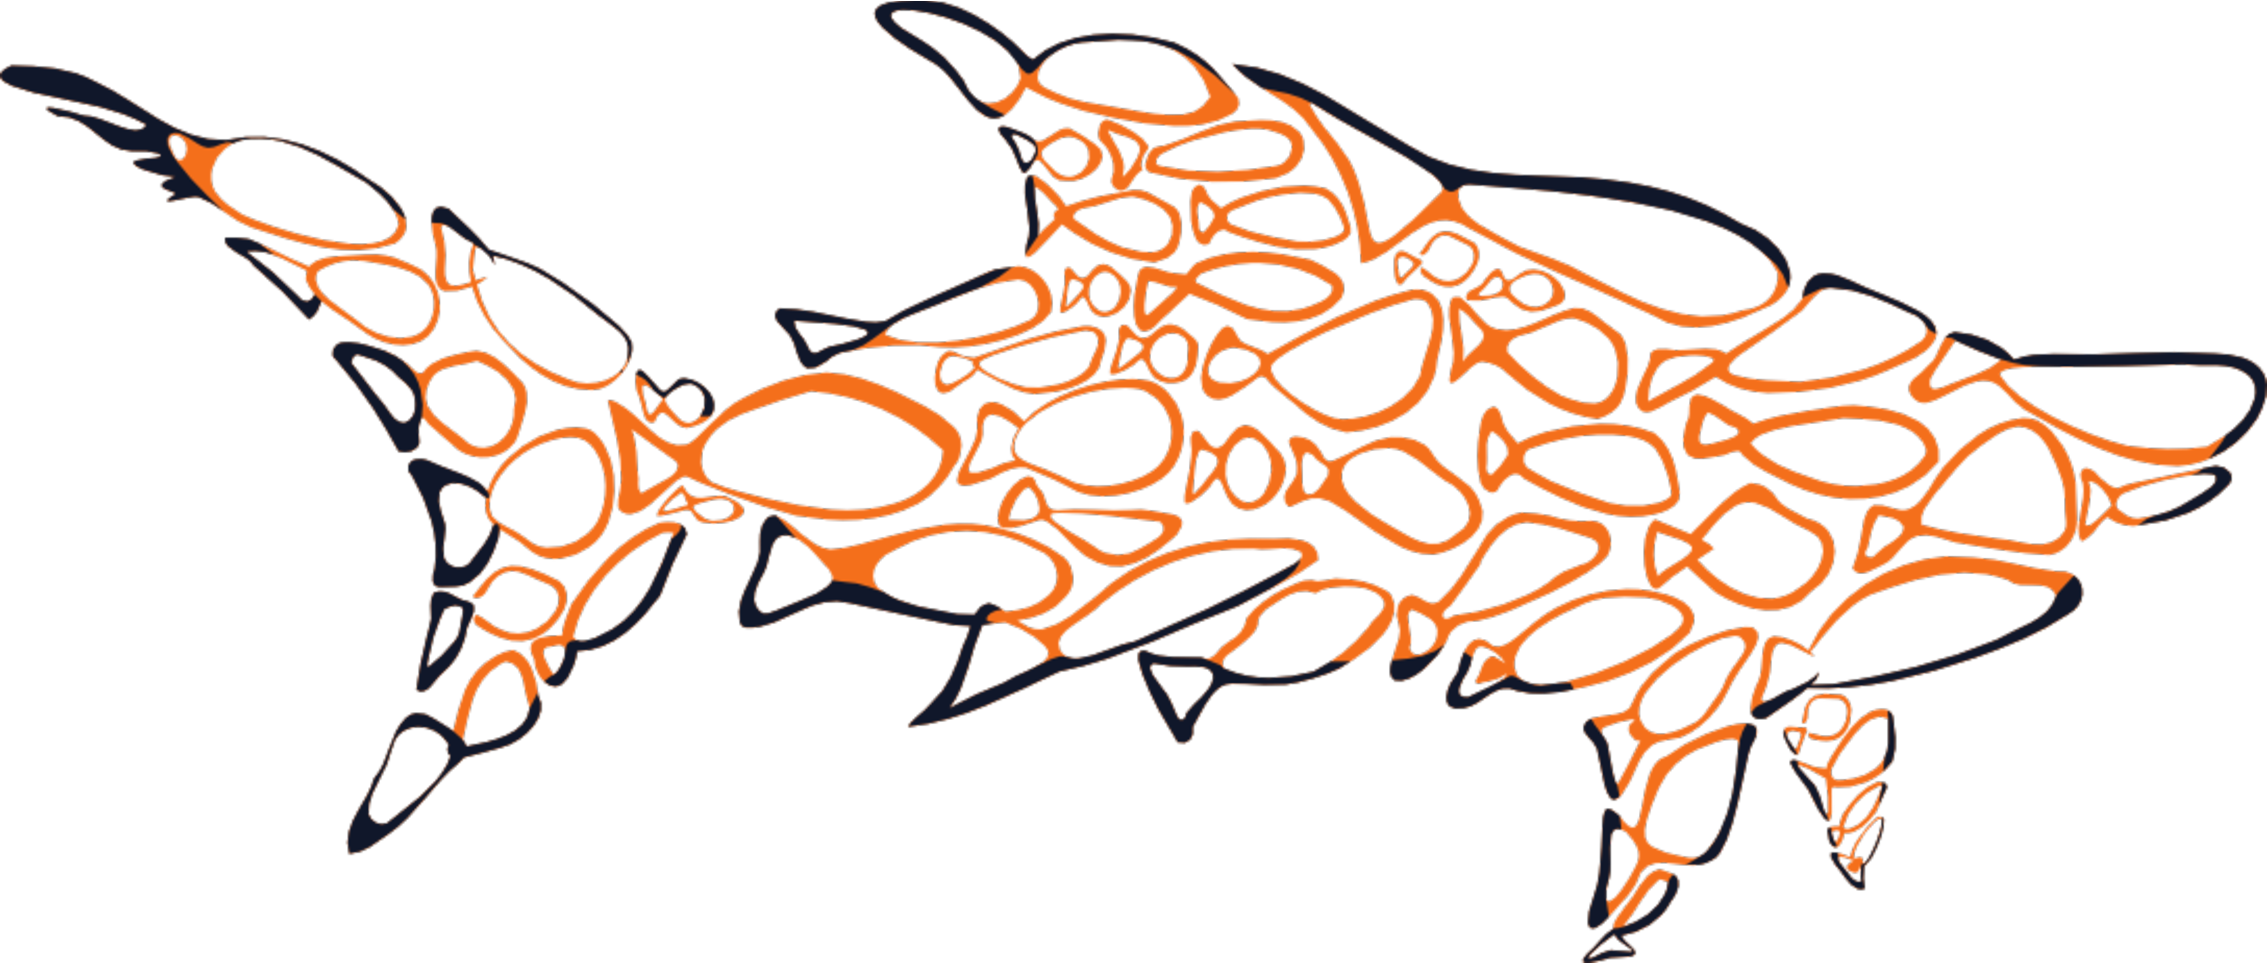
\includegraphics[height=.15\textheight]{./images/i2cvb/shark.pdf}
      \end{figure}
      \vskip-4ex
      \begin{itemize}\tiny
      \item Research groups and individuals from all walks of life to shape a transparent community
      \end{itemize}
    \end{block}
    \column{.5\textwidth}
    \begin{block}{
\includegraphics[height=.04\textheight]{./images/i2cvb/i2cvb.pdf}\ Mission}
      \begin{figure}
        \centering
        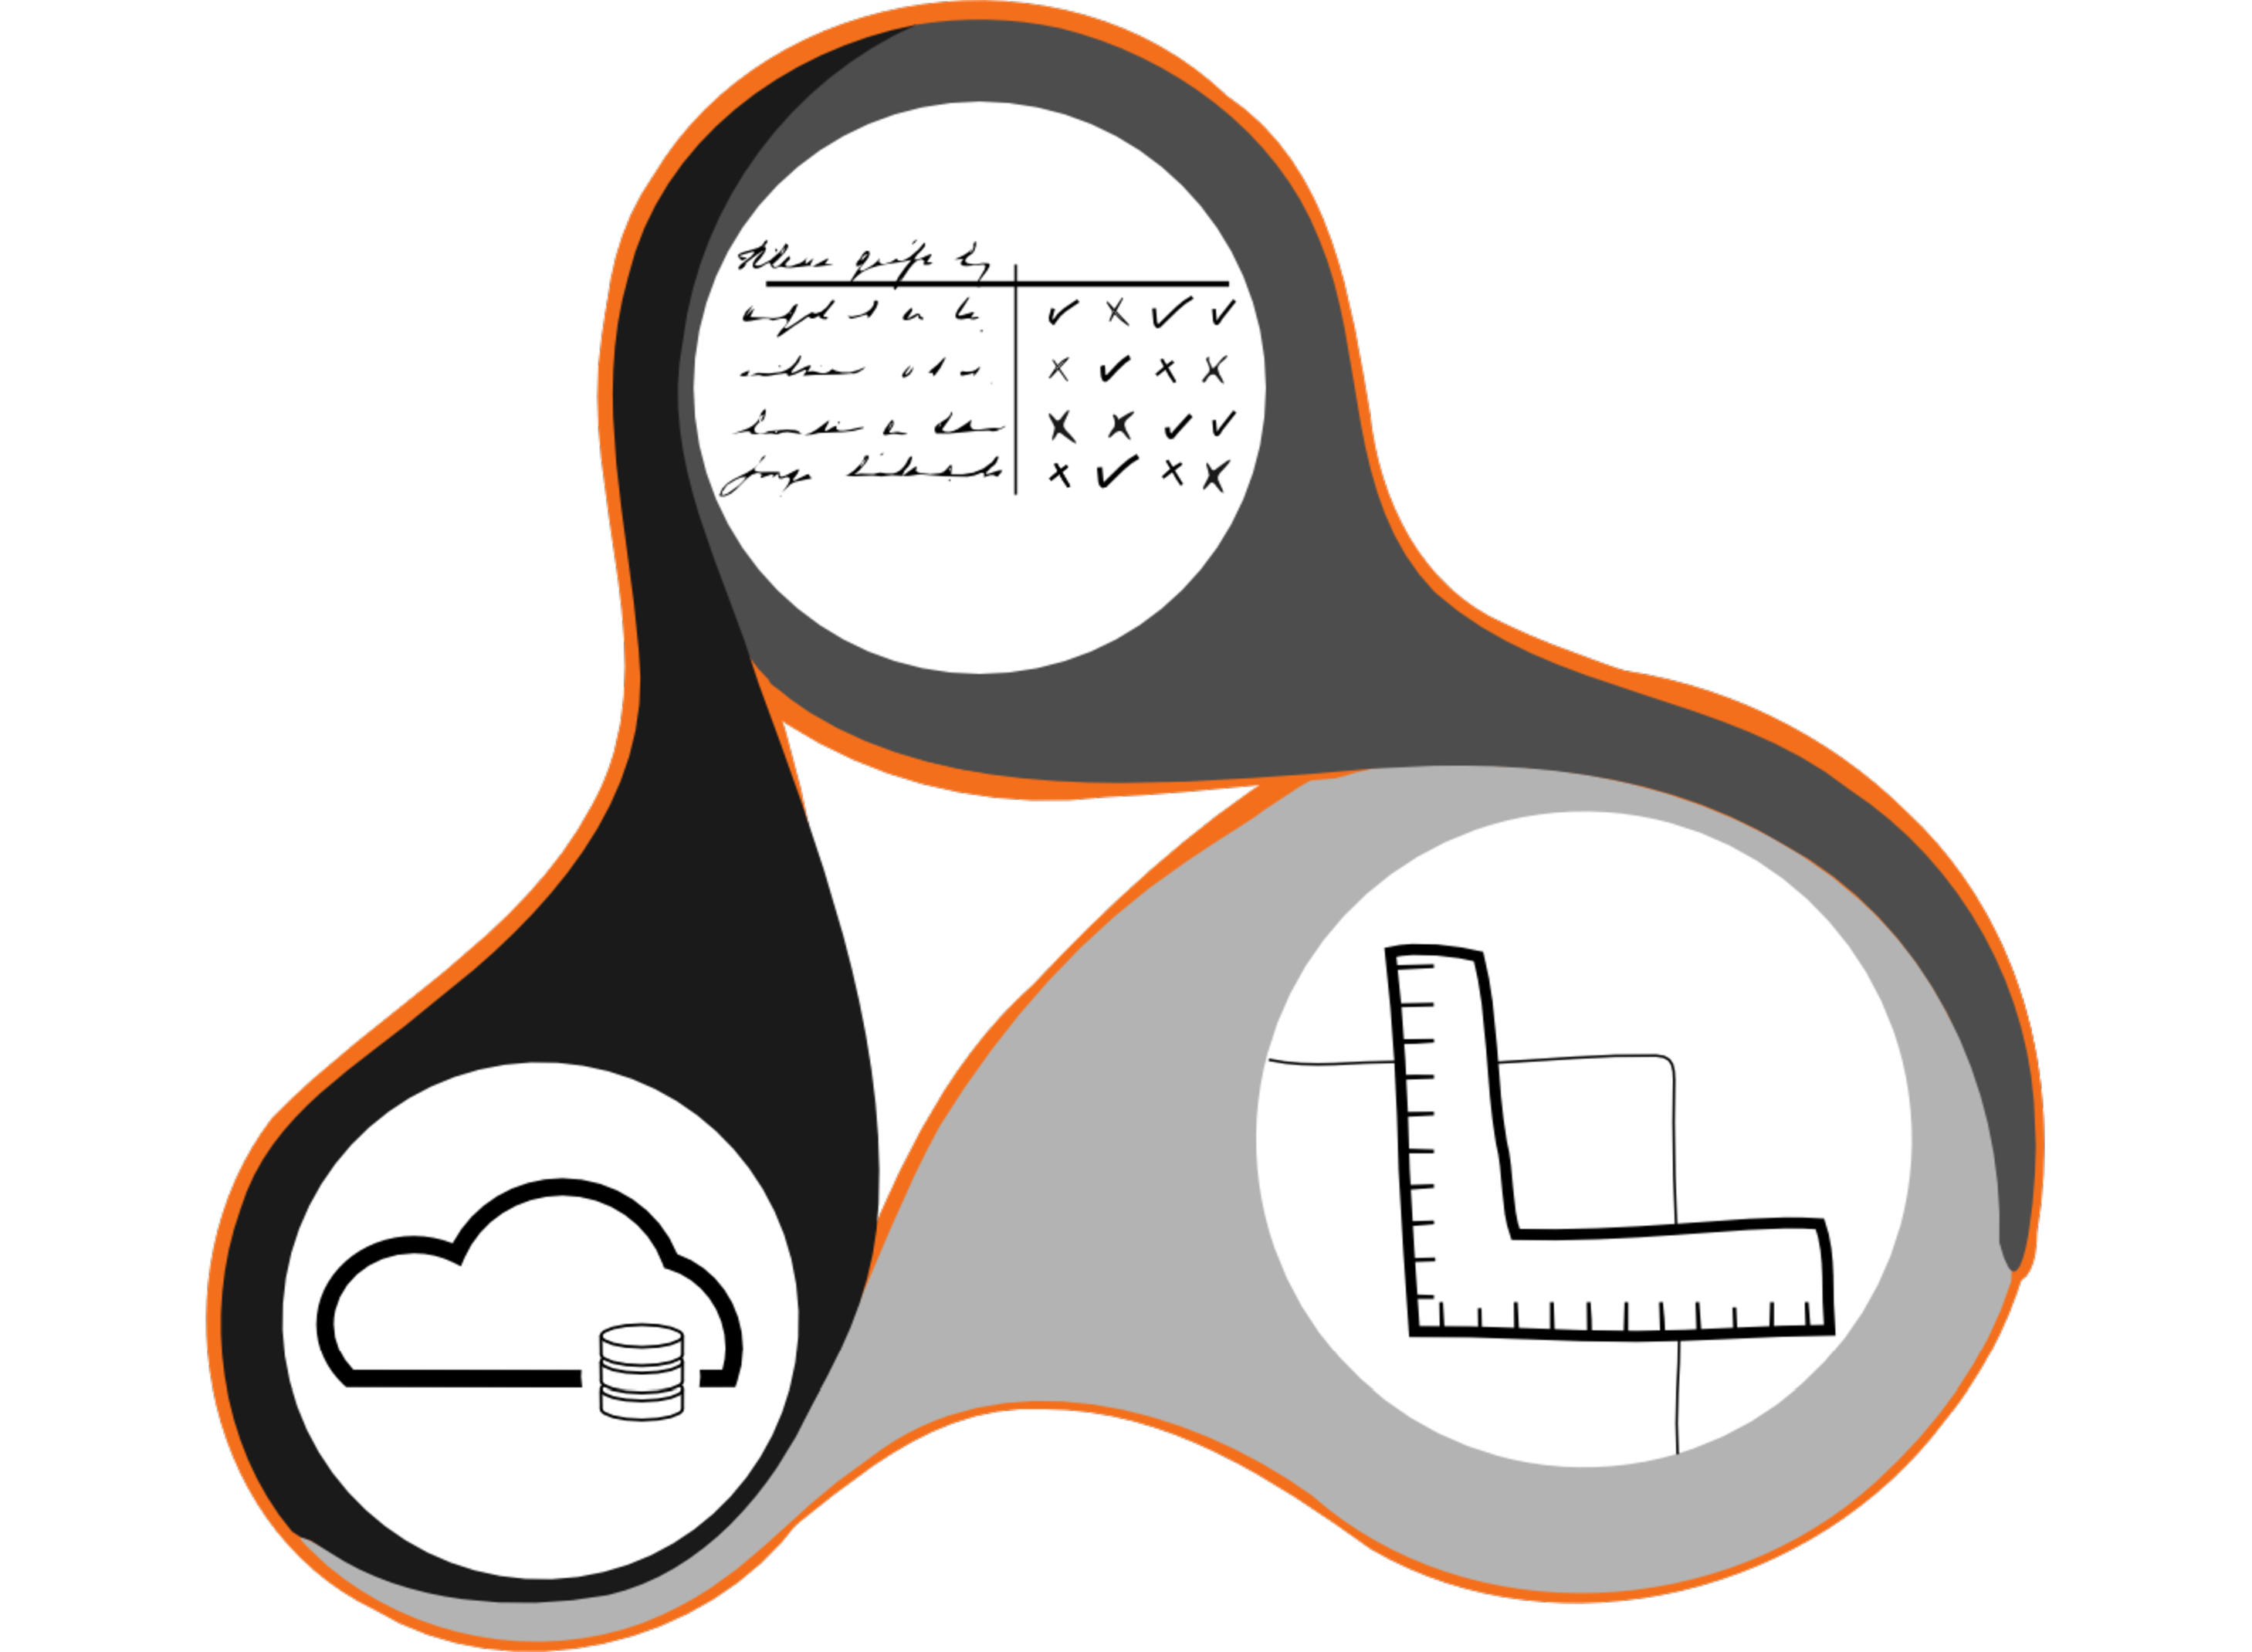
\includegraphics[height=.15\textheight]{./images/i2cvb/what.pdf}
      \end{figure}
      \vskip-4ex
      \begin{itemize}\tiny
      \item Open data; evaluation methods; comparison framework; reporting platform
      \end{itemize}
    \end{block}
    \begin{block}{
\includegraphics[height=.04\textheight]{./images/i2cvb/i2cvb.pdf}\ Strategy}
      \begin{figure}
        \centering
        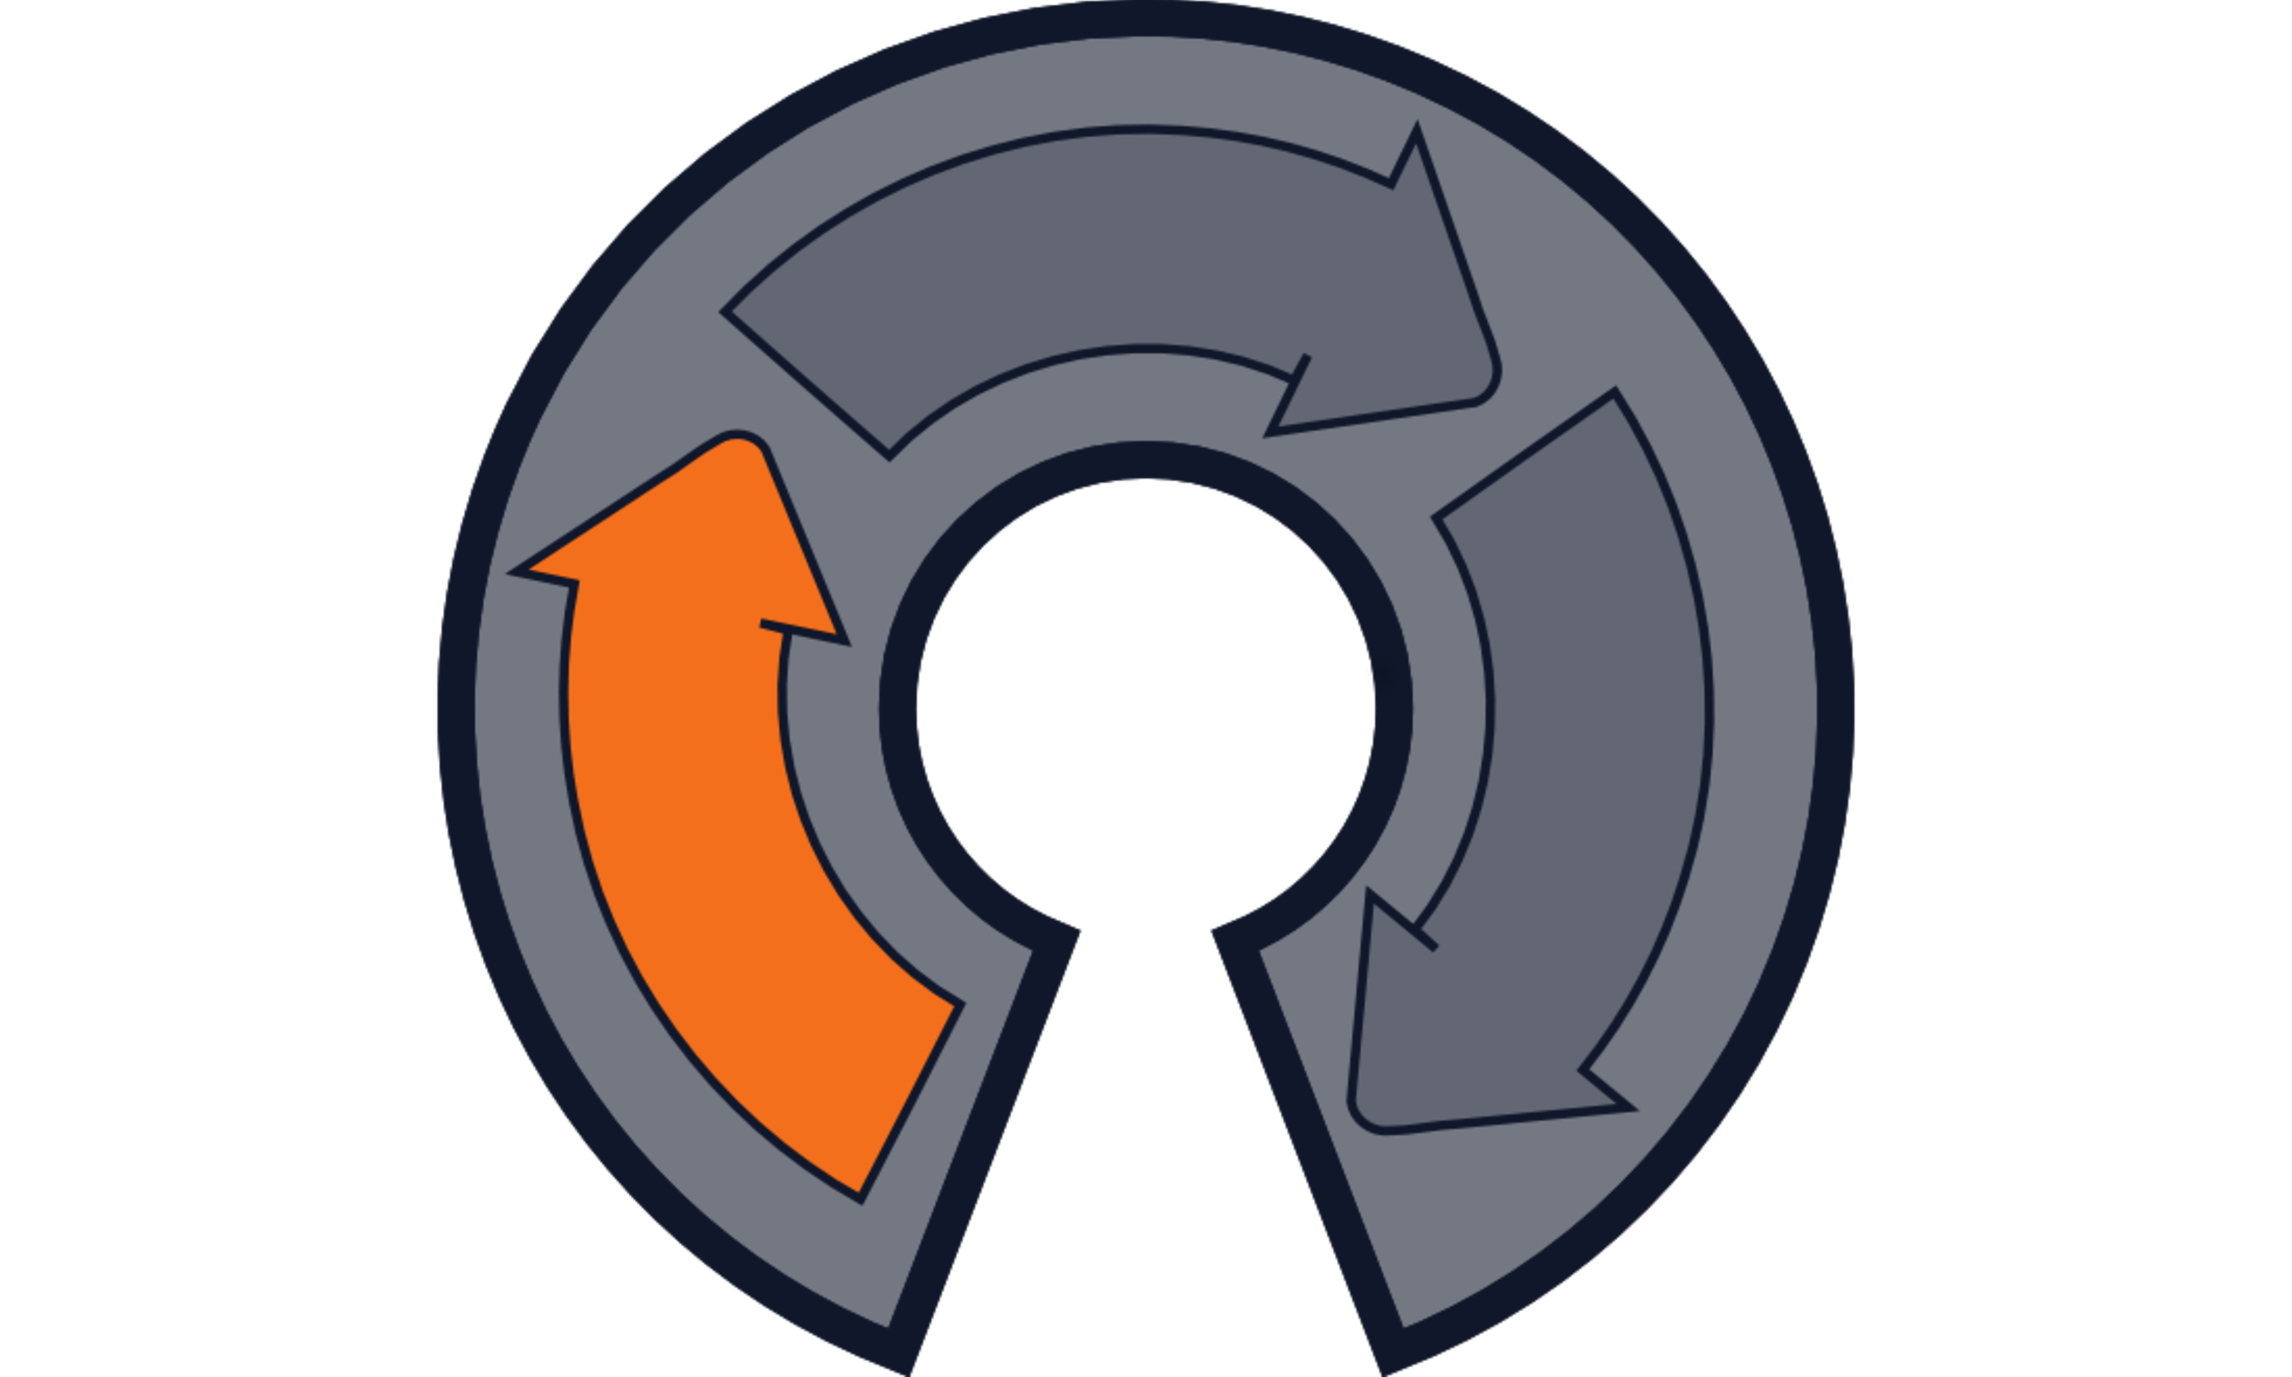
\includegraphics[height=.15\textheight]{./images/i2cvb/open.pdf}
      \end{figure}
      \vskip-4ex
      \begin{itemize}\tiny
      \item Transferring successful practises from Free Software and Quality Management
      \end{itemize}
      \vskip1ex
    \end{block}
  \end{columns}
\end{frame}

\subsection{Prostate dataset}

\begin{frame}
  \frametitle{I2CVB}
  \framesubtitle{Prostate dataset}
  \begin{block}{\small Multi-parametric MRI}\footnotesize
    \begin{itemize}
    \item Cohort of 20 patients
    \item T$_2$W MRI, DCE MRI \& ADC
    \item 3 Tesla whole body MRI without endorectal coil
    \end{itemize}
  \end{block}
  \begin{greenblock}{\small Ground-truth}\footnotesize
    \begin{itemize}
    \item Delineations: prostate - zones - CaP
    \item Healthy: 2 \textit{vs.} CaP: \{PZ: 13, CG: 3, PZ + CG: 2 \}
    \end{itemize}
  \end{greenblock}
\end{frame}

\end{document}